In this chapter we will introduce the basic principles required to understand what waveplates are and how the standard birefringent ones work. Simply put the purpose of a waveplate is to change the polarization of EM waves, most commonly by using a birefringent material. To that extend, the underlying physical principles birefringence and dichroism are explained in more detail in the sections \ref{sec:dichroism} and \ref{sec:birefringence}. Any change to the polarization state caused by the waveplate, and the state itself, can be described mathematically using the Jones calculus which will be shown in section \ref{sec:math_desc}. Finally, this leads to the description of the waveplate design as it is used in this work as well as the design optimization problem which is presented in the last section (\ref{sec:design}) of this chapter.

\section{The polarization ellipse}
\label{sec:polellipse}
There are several ways to describe the polarization state of EM-waves. One of them is the polarization ellipse which is a geometrical representation of the polarization. This remained the only satisfactory way to visualize the different polarization states for almost the entire 19\textsuperscript{th} century, although it is not very practical for carrying out calculations. At the end of the century another representation was proposed by Henri Poincaré, now known as the Poincaré sphere, which could be used for both calculations and visualization of the polarization states \cite{Collett2008VisualizationSphere}. Poincaré's representation will be explained in section \ref{sec:the_poincare_sphere}. The polarization ellipse can be derived either directly from a solution to the EM-wave equation or starting from Maxwell's equations.  It is practical to start from Maxwell's equations, since they are used for derivations later on in this work and almost all equations used originate from them. In differential form Maxwell's equations are given by: 
\par
\noindent\begin{minipage}{.5\linewidth}
\begin{align}
    \bm{\nabla}\cdot\bm{D} &=\rho_{f}\;,\label{eq:maxwell1}
    \vphantom{\frac{\partial\bm{B}}{\partial t}}\\
    \bm{\nabla}\cdot\bm{B} &=0\;,\vphantom{\frac{\partial\bm{B}}{\partial t}}\label{eq:maxwell2}
\end{align}
\end{minipage}%
\begin{minipage}{.5\linewidth}
\begin{align}
    \bm{\nabla}\times\bm{E} &=-\frac{\partial\bm{B}}{\partial t}\;,\label{eq:maxwell3}
    \\
    \bm{\nabla}\times\bm{H} &=\bm{J}_f
    +\frac{\partial\bm{D}}{\partial t}\;,\label{eq:maxwell4}
\end{align}
\end{minipage}
\newline

where $\bm{E}, \bm{H}$ denote the electric and magnetizing fields respectively,  $\bm{D}=\hat{\epsilon} \bm{E}$ is the electric displacement for a linear medium, t is the time and $\hat{\epsilon}$ is the permittivity, which depends on the material and is a complex function of the frequency. The materials used in this work are non magnetic, which means that the magnetic and magnetizing fields are proportional: $\bm{B} = \mu_0 \bm{H}$, where $\mu_0$ denotes the vacuum permeability. $\rho_f, \bm{J}_f$ is the free charge and current density respectively. Usually in optics there are no free charge carriers or free currents, which is also the case for all materials in this work, so we set $\rho_f=\bm{J}_f=0$ \cite{Roth2019Optik}. If we then also assume that the materials are homogeneous so that $\hat{\epsilon}$ does not depend on position, then we can reduce equations \ref{eq:maxwell1}-\ref{eq:maxwell4} to the following:

\noindent\begin{minipage}{.5\linewidth}
\begin{align}
    \bm{\nabla}\cdot \bm{E} &=0\;,\label{eq:maxwell1reduced}
    \vphantom{\frac{\partial\bm{B}}{\partial t}}\\
    \bm{\nabla}\cdot\bm{B} &=0\;,\vphantom{\frac{\partial\bm{B}}{\partial t}}\label{eq:maxwell2reduced}
\end{align}
\end{minipage}%
\begin{minipage}{.5\linewidth}
\begin{align}
    \bm{\nabla}\times\bm{E} &=-\frac{\partial\bm{B}}{\partial t}\;,\label{eq:maxwell3reduced}
    \\
    \bm{\nabla}\times\bm{B} &=\mu_0 \hat{\epsilon} \frac{\partial\bm{E}}{\partial t}\;,\label{eq:maxwell4reduced}
\end{align}
\end{minipage}
\newline

Applying $\bm{\nabla}\times$ to equation \ref{eq:maxwell3reduced} and with equation \ref{eq:maxwell4reduced} we decouple $\bm{E}$ and $\bm{B}$: 
\begin{equation}
    \bm{\nabla}\times \bm{\nabla}\times \bm{E} = -\mu_0 \hat{\epsilon} \frac{\partial^2\bm{E}}{\partial t^2}
\end{equation}
Then using the vector calculus identity: $\bm{\nabla}\times \bm{\nabla}\times \bm{F} = \bm{\nabla} \left( \bm{\nabla} \cdot \bm{F} \right) - \bm{\nabla}^2 \bm{F}$, for any function $\bm{F}$, together with equation \ref{eq:maxwell1reduced} we get the EM-wave equation: \footnote{We neglect the magnetic field, since we are only concerned with non magnetic materials in this work. Nevertheless, the derivation of the wave equation for the magnetic field would be almost exactly the same}
\begin{equation}
    \label{eq:waveeq}
    \bm{\nabla}^2 \bm{E} = \mu_0 \hat{\epsilon} \frac{\partial^2\bm{E}}{\partial t^2}
\end{equation}
and via a Fourier transform $(\partial_t \xrightarrow{\mathscr{F}} i\omega)$ we readily get the Helmholtz equation for $\bm{E}$:
\begin{equation}
    \label{eq:waveeqfreq}
    \bm{\nabla}^2 \bm{E} = -\mu_0 \hat{\epsilon} \omega^2 \bm{E},
\end{equation}
where $\omega$ is the angular frequency.
A solution to the wave equation is a coherent plane wave at frequency $\omega$ which is given by: 
\begin{equation}
    \label{eq:planewave}
    \bm{E} = \bm{E_0} e^{i(\bm{k}\bm{r} - \omega t + \delta)},
\end{equation}
where $\bm{r}$ and $\bm{k}$ denote the position and wave vector respectively, $\bm{E_0}$ denotes the maximum amplitude of the wave and $\delta$ is the phase constant. If we assume the wave propagates along the z-direction in a Cartesian coordinate system, then the amplitude will be orthogonal to the z-direction, i.e a transverse wave. This follows directly from equation \ref{eq:maxwell1reduced}. From the wave equation in frequency space we then find the requirement that the wave number, which is the magnitude of the wave vector, and the angular frequency are related by:
\begin{equation}
    \label{eq:wavevector_req}
    k = \sqrt{\mu_0 \hat{\epsilon}} \omega
\end{equation}
The phase velocity of the wave can then be expressed as:
\begin{equation}
    v = \frac{\omega}{k} = \frac{1}{\sqrt{\mu_0 \hat{\epsilon}}} = \frac{c}{\tilde{n}},\:\tilde{n} = \sqrt{\frac{\hat{\epsilon}}{\epsilon_0}},
\end{equation}
where $c$, $\epsilon_0$ and $n$ is the speed of light in vacuum, vacuum permittivity and refractive index respectively.
So that from the wave equation we get two decoupled wave equations, each describing an oscillation in the x-z plane and the y-z plane. This is also known as Fresnel's wave theory which was proposed and verified experimentally around 1820 by Augustin-Jean Fresnel and François Arago, more than 40 years before Maxwell's equations were published \cite{Collett2009FieldPolarization,Jackson1998ClassicalEdition}.
This means equation \ref{eq:planewave} consists of only two perpendicular components. Additionally, if we consider that Maxwell's equations \ref{eq:maxwell1reduced}-\ref{eq:maxwell4reduced} are all linear and real, then it follows that the real part of any particular solution is also a solution to the wave equation. \footnote{This only works if the equations are real. For example, Schrödinger's equation is linear but complex, therefore even if $\psi$ is a solution $\operatorname{Re}(\psi)$ and $\operatorname{Im}(\psi)$ are not.} We can then write equation \ref{eq:planewave} as two sinusoidal waves:
\begin{equation}
\label{eq:plane_wave_realparts}
\begin{aligned}
    E_x(z, t) = E_{0x}\cos(kz-\omega t + \delta_x) \\
    E_y(z, t) = E_{0y}\cos(kz-\omega t + \delta_y), 
\end{aligned}
\end{equation}
where $\delta_x$ and $\delta_y$ are arbitrary phases of the two components. Depending on the values of $E_{0x}, E_{0y}$ and the relative phase or simply phase, which is $\delta = \delta_y - \delta_x$, we get different polarization states. Figure \ref{fig:Ex_Ey_planewaves} shows the real parts of the two plane wave components for a wave traveling along the z-direction when $\delta=0$ and $E_{0x}=E_{0y}$.

\begin{figure}[h]
    \centering
    \includestandalone{3_chapter03/tikz_e_wave}
    \caption{This figure shows the two sinusoidal waves given in equation \ref{eq:plane_wave_realparts}, which are the real parts of the plane wave components. Both waves have the same amplitude and phase.}
    \label{fig:Ex_Ey_planewaves}
\end{figure}

From here we can visualize the different polarization states, that is the different directions the electrical field, or simply the light, can oscillate in. If the light is confined to a plane along the direction of propagation it is said to be linearly polarized (LP). An example of this is shown in figure \ref{fig:E_planewave}, where the polarization plane is at an angle of \SI{45}{\degree} relative to the x-axis. 

\begin{figure}[h]
    \centering
    \includestandalone[scale=1.1]{3_chapter03/tikz_linear_pol}
    \caption{The black curve shows the superposition of the two sinusoidal waves from equation \ref{eq:plane_wave_realparts}, which is the same as the real part of a LP plane wave at an angle of \SI{45}{\degree} to the x-axis. In addition, the horizontal and the vertical components of the field vector are shown as the red and blue curves respectively.}
    \label{fig:E_planewave}
\end{figure}

Now, if $\delta$ is exactly $\nicefrac{\pi}{2}$ and $E_{0x} = E_{0y}$, then we get the case shown to the right in figure \ref{fig:circ_pol_planewave}. A field with this kind of polarization traces out a circle as time passes for a fixed position in space. On the other hand, if we keep time fixed then the field vector describes a helix along the direction of propagation. This means the field only changes direction but not its magnitude. This type of polarization is therefore called circular polarization (CP). Additionally, because we can trace out a circle in two different directions (clockwise or counterclockwise) we therefore get two different types of circular polarizations. These two types are called left CP (LCP) or right CP (RCP) depending on the direction the circle is traced out, so either in a left- or right-handed sense. This is called the handedness of the light, which can be determined using the right hand rule. For that we fix the right hand at a point on the helix and point the thumb away from the receiver, that is against the direction of propagation. Then the light is right-handed if the helix is traced out in the direction of the other fingers as time revolves, otherwise it is left-handed. The light shown to the left of figure \ref{fig:circ_pol_planewave} is therefore left-handed while the example on the right side of figure \ref{fig:circ_pol_planewave} shows right-handed CP light. The reason why we have two types of CP in the first place, is because of the fact that one component can lead the other, as we can see in figure \ref{fig:circ_pol_planewave}. Where for RCP the horizontal component leads the vertical one by a quarter period ($\delta = -\nicefrac{\pi}{2}$), for LCP it is the other way around and $\delta = \nicefrac{\pi}{2}$. 

\begin{figure}[h]
\centering
    \begin{subfigure}
        \centering
        \includestandalone[scale=0.8]{3_chapter03/tikz_circ_pol_lh}
    \end{subfigure}
    \begin{subfigure}
        \centering
        \includestandalone[scale=0.8]{3_chapter03/tikz_circ_pol_rh}
    \end{subfigure}
    \caption{The left figure shows an example of LCP light and the right figure RCP light. Furthermore, handedness originates from one component leading the other. In the case of LCP light the vertical component leads the horizontal component and vice versa for RCP light.}
    \label{fig:circ_pol_planewave}
\end{figure}

Finally, the last polarization state we have not mentioned yet, even though it is in fact the most general, is the elliptical polarization state. The polarization states we have dealt with so far have all been limiting cases of this state. For a fixed position this is fairly simple to visualize geometrically; LP light traces out a line while CP light traces out a circle, both of these shapes are degenerate forms of an ellipse. A summary of the different degenerate states and the corresponding amplitude and phase combinations are shown in table \ref{tab:pol_state_summary}, which is divided into three parts with a pair of states in each. The linear horizontal/vertical polarization (LHP/LVP) states are at the top, the linear $\pm\SI{45}{\degree}$ polarization ($L_{\pm45}P$) states are in the middle and the CP states are at the bottom. The last column shows the corresponding degenerate ellipse for each state.

\begin{table}[h]
    \centering
    \includestandalone{3_chapter03/pol_summary_table}
    \caption{Summary of the different degenerate polarization states, with corresponding conditions figures. The first four states are linearly polarized at different angles relative to the x-axis; $\SI{0}{\degree}$, $\SI{90}{\degree}$, $\SI{45}{\degree}$ and $\SI{-45}{\degree}$ respectively. The last two are the RCP and LCP states.}
    \label{tab:pol_state_summary}
\end{table}

We can also realize this mathematically by eliminating the time and position dependency of the two components in equation \ref{fig:Ex_Ey_planewaves}, so that we get \footnote{The derivation is given in \ref{sec:deriv_pol_ellipse}}:

\begin{equation}
    \centering
    \label{eq:pol_ellipse}
    \frac{1}{\sin^2 \delta} \left[ \left(\frac{E_x}{E_{0x}}\right)^2+\left(\frac{E_y}{E_{0y}}\right)^2-2\frac{E_x E_y}{E_{0x} E_{0y}}\cos \delta \right]=1,
\end{equation}

which describes an ellipse in its nonstandard form. Because of this the equation is called the polarization ellipse. It is worth noting that even though the time and position dependencies have been explicitly eliminated, the wave components $E_x$ and $E_y$ continue to depend on them. That means $E_{0x}$, $E_{0y}$ and $\delta$ are the polarization ellipse parameters, which then define the shape of the ellipse. Therefore, even though the light propagates the shape remains constant. There are several ways to parameterize the polarization ellipse or ellipses in general using two variables. One way is to use the orientation angle $\psi$ and the ellipticity angle $\chi$, which both can be expressed through the polarization ellipse parameters: 

\begin{equation}
    \label{eq:ellipse_orientation}
    \tan 2\psi = \frac{2E_{0x}E_{0y}}{E_{0x}^2 - E_{0y}^2}\cos \delta,\: 0\leqslant\psi\leqslant\pi,
\end{equation}
\begin{equation}
    \label{eq:ellipse_ellipticity}
    \sin 2\chi = \frac{2E_{0x}E_{0y}}{E_{0x}^2 + E_{0y}^2}\sin \delta,\: \nicefrac{-\pi}{4}\leqslant\chi\leqslant\nicefrac{\pi}{4}.
\end{equation}
Figure \ref{fig:pol_ellipse} shows an example of a polarization ellipse together with the orientation and ellipticity angles. We see from the figure that for $\psi \rightarrow 0/\pi$ or $\psi \rightarrow \nicefrac{pi}{2}$ the major and minor axes $(a$ and $b)$ coincide with the coordinate axes. Likewise for $\chi \rightarrow 0$ the ellipse degenerates to a line and for $\chi \rightarrow \pm\nicefrac{\pi}{4}$ we get a circle \cite{Collett2009FieldPolarization}. Actually, in most cases a light beam is a mixture of different polarization states, this is referred to as unpolarized light. It consists of a high number of short wave trains which are emitted from the individual atoms. In most cases these wave trains are radiated from dipoles and are therefore linearly polarized, but since every atom oscillates in a different direction the polarization will also vary for each wave train. Hence, the beam will be a mixture of different states \cite{Roth2019Optik}. 

\begin{figure}[h]
    \centering
    \includestandalone[scale=1.1]{3_chapter03/tikz_pol_ellipse}
    \caption{Example of a polarization ellipse, which shows the ellipticity and orientation angle geometrically. The major and minor axes of the polarization ellipse are denoted by $a$ and $b$ respectively. We see that $\chi$ changes with the shape of the ellipse while $\psi$ is simply the orientation relative to the x-axis.}
    \label{fig:pol_ellipse}
\end{figure}

We finish off this section, as a bit of a side note, by mentioning the conventions used so far. If we go back to the plane wave solution (equation \ref{eq:planewave}) of the wave equation we see that a replacement of $i$ with $-i$ yields another valid linearly independent solution. This leads to two different sets of definitions, depending on the of the imaginary unit. The first one, with a positive sign and the one used here, is commonly used in physics texts. While the other one with a negative sign is mainly used in electrical engineering (EE) texts. Mathematically the difference between these two conventions is simply the direction of rotation of the phasor in the complex plane with increasing time. An example of this is shown for a phasor $x$ in figure \ref{fig:phasor}. 

\begin{figure}[h]
    \centering
    \includestandalone[scale=1.3]{3_chapter03/tikz_phasor_rotation}
    \caption{Example of a phasor $x$ in the complex plane. The sign of the imaginary unit determines the direction of rotation for increasing times. The rotation is indicated by the blue arrows and is either in the clockwise $(-i)$ or counterclockwise $(+i)$ direction.}
    \label{fig:phasor}
\end{figure}

The choice of sign has other implications. We know from equation \ref{eq:wavevector_req} that the wavevector is in general complex because the permittivity is, so we can write it as $k=\beta + i \alpha$. On the other hand we get two expressions for a plane wave propagating in the z-direction, one for each definition:
\begin{align}
    &\bm{E_{0}}e^{i((\beta + i \alpha)z-\omega t + \delta)} \\
    &\bm{E_{0}}e^{-i((\beta + i \alpha)z-\omega t + \delta)}, 
\end{align}
if we factor out the $\alpha$ dependency we get:
\begin{align}
    e^{-\alpha z}&\bm{E_{0}}e^{i(\beta z-\omega t + \delta)} \\
    e^{\alpha z}&\bm{E_{0}}e^{-i(\beta z-\omega t + \delta)}. 
\end{align}
We see that in case of the EE definition the amplitude would increase as the wave propagates, which is nonsense.\footnote{This problem also arises in the derivation of the Lorentz oscillator model. More about this in the appendix (section \ref{sec:lorentz_model_sign}), since it is out of scope of this work.} Therefore the sign of the imaginary part of the wavevector must be chosen accordingly. So for the EE definition we get:
\begin{equation}
    k=\beta - i \alpha
\end{equation}
and 
\begin{equation}
    k=\beta + i \alpha
\end{equation}
for the physics definition.
As a result the sign of the imaginary part of the refractive index will also depend on the chosen definition. When the EE definition is used:
\begin{equation}
    \tilde{n}= n - i \kappa
\end{equation}
and using the physics definition:  
\begin{equation}
    \tilde{n}= n + i \kappa.
\end{equation}

The physics definition is used for example in the textbooks by John D. Jackson \cite{Jackson1998ClassicalEdition} and David J. Griffiths \cite{Griffiths2017IntroductionElectrodynamics} and also in \cite{Collett2009FieldPolarization}, which is the reference used for most of this section.
There are not only convention differences between engineers and physicists but also even between different branches of physics. The definition of CP handedness relies on the point of view; that is either looking from the source in the direction of propagation or from the receiver against the direction of propagation. Here we use the version which is defined from the point of view of the receiver. This is also the convention commonly used in optics \cite{Bass2016HandbookOptics, M.LandiDeglInnocenti2004PolarizationLines} as well as by SPIE \cite{Collett2009FieldPolarization}.
The other convention is used by radio astronomers \cite{1973CommissionAstronomie}, quantum physicists, because it is consistent with the convention of handedness for a particle's spin and it is also used by electrical engineers \cite{Orfanidis2004ElectromagneticAntennas}.

\section{Wave propagation in anisotropic media}
In the previous section we saw that the electrical field consists of two perpendicular components which trace out an ellipse as time propagates for any fixed position. Additionally, the shape and orientation of the ellipse depends on the relative phase of the two components as well as their amplitudes. Naturally this dependency is symmetrical in the two amplitudes and the relative phase, as can be seen directly from equations \ref{eq:ellipse_orientation} and \ref{eq:ellipse_ellipticity}. Therefore in order to change the polarization state, the change in each of the individual phases must be different and or that of the two amplitudes. Otherwise simply the scale of the ellipse would change and not its shape or orientation. Consequently, for this to happen the medium the wave is propagating in must be anisotropic. Now, if the absorption of the material is direction dependent, then the amplitude will vary differently for the two components. Materials with this property are said to be dichroic. Likewise, some materials cause different phase changes between the two components. This material property is called birefringence. In the following section we will explain these two properties phenomenologically as well as their underlying physical principle.

\subsection{Dichroism}
\label{sec:dichroism}
In general, the term dichroism refers to the selective absorption of one of the two perpendicular field components of the light. Materials with this property are said to be dichroic. This can be used in for example polarizers, which are extremely anisotropic so that one component is almost completely extinguished by the polarizer, while it is transparent to the other field component. The simplest polarizer of this sort is a grid of parallel conducting wires as it is shown in figure \ref{fig:wire_grid_polarizer} which is also known as a wire grid polarizer (WGP). The WGP is similar to a conducting diffraction grating with a sub-wavelength period. Now, if we assume that the light initially is unpolarized as it propagates towards the wire grid from the left, then the light will be linearly polarized perpendicular to the wires after the WGP. We can see this by considering the interaction of the two field components with the wires separately. One component can then be set to be parallel to the wires and the other perpendicular. The electrons are free to move in the y-direction, because the wires are conducting, so that a current is generated due to the acceleration of the electrons by the parallel field component. This current results in joule heating of the wires so that a part of the energy of the electric field is turned into heat. Additionally, the accelerated electrons radiate in both the forward and backward directions. The part that is radiated forwards, along the direction of propagation, mostly cancels the transmitted incident wave and the other part appears as the reflected wave. On the other hand, the electrons along the x-direction, that is perpendicular to the wires, are not free to move very far so that the corresponding wave component passes almost freely. So, at the end the component parallel to the wires is mostly extinguished and the light is therefore linearly polarized perpendicular to the wires \cite{HechtOpticsEdition}.

\begin{figure}[h]
    \centering
    \includestandalone[scale=1.30]{3_chapter03/tikz_wire_grid_polarizer}
    \caption{This figure shows a wire grid polarizer which is essentially a conducting sub-wavelength grating. From the left unpolarized light interacts with the wire grid so that the field components parallel to the wires are eliminated. After passing the polarizer the light is therefore linearly polarized perpendicular to the wires.}
    \label{fig:wire_grid_polarizer}
\end{figure}

It has been shown that it is possible to polarize even visible light using these wire grids. In 1960 George R. Bird and Maxfield Parrish fabricated a WGP having 2160 wires per mm, making it suitable for Near-Infrared light \cite{Bird1960ThePolarizer}. Naturally, WGPs also exist for the lower THz-range. An example of this is an aluminum-based WGP with a frequency range of \SIrange{0.3}{2.5}{\tera \hertz} and an extinction ratio ranging from \SI{45}{\dB} for lower frequencies and \SI{30}{\dB} for the higher ones. The extinction ratio is simply the ratio of the transmitted power coefficients for the field components perpendicular and parallel to the wires in decibel, so it is a measure of how well the light is only transmitted perpendicular to the wires after passing the polarizer \cite{Ferraro2016FlexibleLoss}. 
In contrast to a WGP some materials are inherently dichroic. For example the mineral tourmaline has a specific axis, which in general is called the optic axis. Light propagating parallel to this axis experiences a smaller absorption coefficient compared to any other direction. Additionally, this selective absorption depends on the wavelength of the light. Therefore if the crystal is illuminated with white polarized light, then the absorbed colors will change depending on the polarization and so the crystal will change color depending on the polarization. This is where the name dichroic comes from, meaning two colors. The mechanism that gives rise to dichroism in crystals can be explained by considering its microscopic structure. The electrons bound to the lattice points of the crystal interact with electrons bound to other nuclei, especially the nearest neighbors. So if the crystal lattice is asymmetrical then the binding forces of the electrons will also be asymmetrical resulting in a polarization dependent response. Additionally, if the conductivity depends on the direction so will the amount of joule heating generated due to the induced currents. As a consequence the absorption will be direction dependent. To summarize, in this section we discussed two types of dichroism; one originating from a non-zero anisotropic conductivity of the structure on a macroscopic scale explained using the example of a WGP and the other type arising from asymmetries on the atomic scale. Loosely speaking, the effects of dichroism and birefringence in the cases relevant for this work can be explained by a direction and polarization dependent imaginary and real part of the refractive index respectively. This complicates the description of em-wave propagation in anisotropic materials, as we will see in the following section which introduces the most relevant concepts related to birefringence \cite{HechtOpticsEdition}.

\subsection{Birefringence}
\label{sec:birefringence}
Birefringence is the material property responsible for the phenomenon of double refraction. This phenomenon was observed for the first time in calcite crystals by the Danish scientist Rasmus Bartholin in 1669 \cite{RasmusBartholin1669ExperimentaDetegitur, Restaino2015PolarizationDevices}. The effect of double refraction on a light beam passing through a birefringent material is relatively easy to show. One can simply place a birefringent crystal on top of some text, as it is shown in figure \ref{fig:3birefringence}. Two images of the text become visible through the crystal and each image is shifted by a different amount. These images are not simply reflections at the crystal-air interface, since the images are brighter compared to images formed through reflections, and they are even visible when looking down directly from above. Also if the crystal is rotated then one of the images will be stationary, while the other one will circle around the stationary image. The waves forming the stationary image are known as the ordinary waves (o-rays or o-waves) and combined they form the o-wave, while the ones forming the moving image are called extraordinary waves (e-rays or e-waves) as suggested by Bartholin at the discovery of the phenomena. The same effect can be illustrated by sending an unpolarized laser beam through the crystal. The beam is split in two as it propagates through the crystal. One can show, using a WGP or any other polarizer, that the polarization states of the two beams are orthogonal \cite{Roth2019Optik}.

\begin{figure}[h]
    \centering
    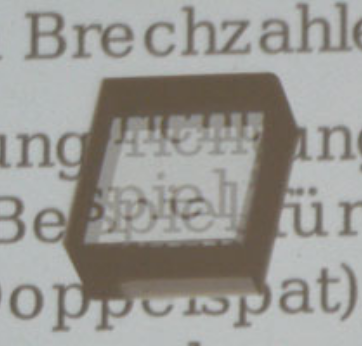
\includegraphics[scale=0.25]{images/3_chapter03/birefringence.png}
    \caption{A calcite crystal placed on top of some text. This demonstrates the effect of birefringence on the original image seen through the crystal \cite{Roth2019Optik}.}
    \label{fig:3birefringence}
\end{figure}

The explanation of the underlying physical principle of birefringence is similar to that of dichroism; it can be explained by considering the structure of the material. We can represent the binding of the electron cloud to the nuclei at each crystal lattice point using a harmonic oscillator model. The model, which is shown in figure \ref{fig:electron_shell}, consists of a shell bound to the nuclei with springs. Furthermore, the springs have different spring constants and the nuclei is fixed in space. So, if an electron is displaced parallel to one of the springs it will oscillate with a different frequency relative to any other direction. How this finally influences the refractive index can be explained by considering the propagation of light through a transparent medium. As the wave propagates through the medium the electrical field excites the electrons which then in turn reradiate because any accelerating charge emits radiation. These reradiated wavelets recombine to form the refracted wave. Additionally, the phase velocity of the refracted wave will be determined by the frequency difference between the natural oscillation of the electrons and the frequency of the electrical field. Since the refractive index is simply the ratio between the speed of light in vacuum and in the medium it will change too depending on this frequency difference. If we go back to figure \ref{fig:electron_shell} this means that for example a wave linearly polarized parallel to the x-axis experiences a different refractive index compared to one polarized parallel to the z-axis. That is also the definition of birefringence; a material with two or more different refractive indices. At this point it is worth making a few general remarks about this mechanical spring model in the following part before we continue. It is called the Lorentz oscillator model after Hendrik Antoon Lorentz who first devised this theory in the late nineteenth century. This was before the discovery of quantum mechanics and it was therefore originally purely a classical model. The model was then later adapted to quantum mechanics and is still often used to describe the interaction between atoms and electric fields. Lorentz did not assume that the electron actually was bound to the nucleus by a physical spring but rather that the force could be approximated by a harmonic oscillator. This is a justified assumption since any kind of binding force can be approximated by a harmonic oscillator, if the displacement is small enough so that only the linear terms in the Taylor expansion are significant. However, this classical version of the model fails at explaining a large number of the observed effects, especially when a weak field is interacting with a small number of atoms. For this situation and others, at least a partially quantum mechanical description is required. As an example, in \cite{Rerat2020FromApproach} the birefringence is calculated using a quantum mechanical treatment \cite{doi:https://doi.org/10.1002/9780470409718.ch3}. Now, for the rest of this section we will explain the phenomena described at the start of the section and then introduce a few more useful concepts to finish off the section. A concept that is helpful in understanding the phenomena is the optic axis of a crystal\footnote{In the context of crystals it is called the optic axis, otherwise it is called the optical axis like the axis perpendicular to the center of a lens \cite{HechtOpticsEdition}.}. That is, if we have the case in which two springs have the same rigidity, for example those in the xy-plane, then the optic axis will be parallel to the z-axis. The special property of the optic axis is that any wave propagating parallel to it will not undergo any birefringence effects, because the material is optically symmetrical under any rotation about this axis. Therefore the two components of the wave, which are also perpendicular to the direction of propagation, will experience the same refractive index. Since this symmetry exists at every lattice point, the optic axis is actually a direction and not just a line through a single point \cite{HechtOpticsEdition}. 

\begin{figure}[h]
    \centering
    \includestandalone[scale=0.9]{3_chapter03/tikz_electron_shell}
    \caption{Lorentz oscillator model of an electron cloud, which is represented by a negatively charged spherical shell. It is bound to its positively charged nucleus via springs of different strength. The mass of the nucleus is assumed to be infinite so that it is fixed in space. This model is a simplification of an optical anisotropic material, for an isotropic material the spring constants would all be equal.}
    \label{fig:electron_shell}
\end{figure}

Furthermore, this explains the phenomena described at the beginning of this section. Going back to the calcite crystal shown in figure \ref{fig:3birefringence} we see that the optic axis must be at an angle, not parallel or perpendicular, to the surface normal. Otherwise we would not observe double refraction. Additionally, the field components perpendicular to the optic axis will not be refracted and therefore form the o-waves, which makes the image look like it is seen through an ordinary piece of glass. The other field components will have a part parallel to the optic axis and one perpendicular to it. This means that the wavefront gets distorted and that part is therefore refracted. Those refracted parts then form the e-wave. Finally, this also explains why the polarizations states of the o- and e-waves are orthogonal because of the spatial separation of the two field components. For clarity a sketch of the field, as it passes through the calcite crystal, is shown in figure \ref{fig:calcite_beams}. A crystal with exactly one symmetry axis or optic axis like calcite is said to be uniaxial. Crystals with two optic axes also exists, i.e. the case shown in figure \ref{fig:electron_shell} where the springs in the x-, y- and z-directions all differ, these crystals are called biaxial but we will not encounter them in this work. 

\begin{figure}[h]
    \centering
    \includestandalone[scale=0.95]{3_chapter03/tikz_calcite_beams}
    \caption{The field components are separated as the light passes through the calcite crystal thereby forming the e- and o-wave. The components perpendicular to the optic axis shown as red dots pass through as expected for normal incidence, while the other components represented by the blue arrows are refracted. It also explains why the polarization states of the two waves are orthogonal.}
    \label{fig:calcite_beams}
\end{figure}

Figure \ref{fig:uniaxial_source} shows the propagation of a wave emitted from an unpolarized source placed within a uniaxial crystal. The component of the field perpendicular to the optic axis will propagate with the same phase velocity $v_{\bot}$ in all directions, so that the wavefronts form the o-wave which further expands in the shape of a circle. Meanwhile the field component, which is not everywhere perpendicular to the optic axis, will be traveling with a phase velocity $v_{\parallel}$ in the directions perpendicular to the optic axis. The wavefronts of the e-wave therefore form an ellipse. We therefore end up with different refractive indices with extrema along and perpendicular to the optic axis. In this case the highest refractive index $n_o = \nicefrac{c}{v_{\bot}}$ is found in the directions parallel to the optic axis, while it is lowest for the perpendicular directions. Because $v_{\parallel} > v_{\bot}$ and since the refractive index perpendicular to the optic axis is given by $n_e = \nicefrac{c}{v_{\parallel}}$ it follows that $n_e < n_o$. With this it is possible to quantify the birefringent strength of the material via the difference $\Delta n = n_e - n_o$ in the refractive indices of the o- and e-wave. The difference $\Delta n$ is known as the birefringence of the material. Furthermore, if $\Delta n$ is negative then the crystal is said to be negative uniaxial which is the case for calcite and the example shown in figure \ref{fig:uniaxial_source}. Likewise, if $\Delta n$ is positive the material is positive uniaxial and in that case the ellipse formed by the wavefronts of the e-wave are enclosed within the circle formed by the wavefronts of the o-wave. 

\begin{figure}[h]
    \centering
    \includestandalone[scale=0.73]{3_chapter03/tikz_uniaxial_source}
    \caption{Cross section perpendicular to the optic axis of an unpolarized light source inside a uniaxial crystal. The red dots represent components which are everywhere perpendicular to the optic axis. They form the o-wave and expand in a circle because they experience the same refractive index everywhere. The components represented by the blue arrows are partly pointing in the direction of the optic axis. Therefore, depending on their orientation to the optic axis they experience a different refractive index so that the wavefront forms an ellipse.}
    \label{fig:uniaxial_source}
\end{figure}

For biaxial crystals birefringence is still defined as the biggest difference between the refractive indices along the different directions. For completeness, it is worth mentioning the case in which the refractive indices along all the directions are equal. The unit cell of these materials is cubic causing them to be isotropic \cite{HechtOpticsEdition}. 
Finally, to conclude this section we will give a description of the same situation but from another point of view. To that extend we consider the energy density of an em-wave in an anisotropic medium.
We start by introducing a charge density $\rho$ and then express the work done by the fields moving it a distance $d\bm{l}=\bm{v}dt$ in terms of the fields themselves. Since that gives us an idea of the energy stored in the fields. The force acting on the charge distribution is the Lorentz force density\footnote{The force density has the dimensions of force per volume and is needed so that when we integrate over the volume we get the total force.} $\bm{f}$:
\begin{equation}
    \bm{f}\cdot d\bm{l}=\rho(\bm{E}+\bm{v}\times\bm{B})\cdot\bm{v}dt=\rho\bm{E}\cdot\bm{v}dt
\end{equation}
We get the last equality because $\bm{v}\cdot(\bm{v}\times\bm{B})$ is zero for any $v$ and $\bm{B}$. 
If we then integrate over the volume $V$ enclosing the charge distribution and use the fact that $\bm{J}=\rho\bm{v}$ we get:
\begin{equation}
    \int_V \bm{f}\cdot d\bm{l} dV =\int_V \bm{E}\cdot\bm{J} dVdt
\end{equation}
since $\int_V \bm{f} dV = \bm{F}$ and $dW = \bm{F} d\bm{l}$ we finally end up with:
\begin{equation}
    \label{eq:emf_work}
    \frac{dW}{dt} = \int_V \bm{E}\cdot\bm{J} dV
\end{equation}
Since we want to express this in terms of the fields only we use the Ampère-Maxwell law, that is equation \ref{eq:maxwell4}:
\begin{equation}
    \bm{J}\cdot\bm{E} = \frac{1}{\mu_0}\bm{E}\cdot(\bm{\nabla}\times\bm{B})-\bm{E}\cdot\frac{\partial\bm{D}}{\partial t}
\end{equation}
We can rewrite $\bm{E}\cdot(\bm{\nabla}\times\bm{B})$ as $-\bm{B}\cdot\frac{\partial \bm{B}}{\partial t} - \bm{\nabla}\cdot(\bm{E}\times\bm{B})$ using a product rule from vector calculus and the Maxwell–Faraday law (equation \ref{eq:maxwell3}). With the fact that $\bm{A}\cdot\frac{\partial \bm{A}}{\partial t} = \frac{1}{2} \frac{\partial A^2}{\partial t}$ for any vector $\bm{A}$ we finally end up with:
\begin{equation}
    \bm{J}\cdot\bm{E} = -\frac{1}{2}\frac{\partial}{\partial t}\left(\frac{1}{\mu_0}B^2+\bm{E}\cdot\bm{D}\right)-\frac{1}{\mu_0}\bm{\nabla}\cdot(\bm{E}\times\bm{B})
\end{equation}
which we then substitute back into equation \ref{eq:emf_work} and with the help of the divergence theorem we get:
\begin{equation}
    \label{eq:poyntings_theorem}
    \frac{dW}{dt} = -\frac{\partial}{\partial t} \int_V \frac{1}{2}\left(\frac{1}{\mu_0}B^2+\bm{E}\cdot\bm{D}\right)dV -\frac{1}{\mu_0}\oint_{\partial V} (\bm{E}\times\bm{B}) \cdot d\bm{s}
\end{equation}
This is known as Poynting's theorem in integral form and can be compared to the work-energy theorem of classical mechanics. That is, the work done by an electromagnetic force on a charge distribution equals the decrease of energy stored in the fields. The volume integral of equation \ref{eq:poyntings_theorem} is the total energy stored in the fields while the surface integral describes the energy flux or rate of transport out of the volume by the fields. We can therefore rewrite equation \ref{eq:poyntings_theorem} as:
\begin{equation}
    \frac{dW}{dt} = -\frac{\partial}{\partial t} \int_V u\, dV -\oint_{\partial V} \bm{S} \cdot d\bm{s}
\end{equation}
where we have set
\begin{equation}
    u = \frac{1}{2}\left(\frac{1}{\mu_0}B^2+\bm{E}\cdot\bm{D}\right),\; \bm{S} = \frac{1}{\mu_0}(\bm{E}\times\bm{B}),
\end{equation}
$u$ is the energy density of the fields and $\bm{S}$ is the energy flux density known as the Poyinting vector. Since we have no free charges for the cases considered in this work, that is free space or neutrally charged media, we set $\frac{dW}{dt}=0$. With equation \ref{eq:emf_work} we get the differential form:
\begin{equation}
    \label{eq:poynting_theorem_diff_form}
    \frac{\partial u}{\partial t} = -\bm{\nabla} \cdot \bm{S},
\end{equation}
because the volume integral (equation \ref{eq:emf_work}) is zero for any volume. We see that \ref{eq:poynting_theorem_diff_form} has the same shape as a continuity equation like the heat flow equation or the continuity equation in quantum mechanics related to the conservation of probability, in this case it shows that energy is conserved locally. Finally, if we take only the electric field contribution to the energy density, that is $u_e = \frac{1}{2}\bm{E}\cdot\bm{D}$, and choose a coordinate system in which the dielectric tensor is diagonal, known as the principal coordinate system, then we can write the electrical displacement vectors for which $u_e$ is constant as:
\begin{equation}
    \frac{D_x^2}{\epsilon_x}+\frac{D_y^2}{\epsilon_y}+\frac{D_z^2}{\epsilon_z}= 2u_e
\end{equation}
where $\epsilon_x$, $\epsilon_y$ and $\epsilon_z$ are the dielectric constants on the diagonal of $\hat{\epsilon}$ called the principal dielectric constants. Additionally we scale $\bm{D}$ by $\nicefrac{1}{\sqrt{2u_e}}$, replace it with $\bm{r}$ and set $n_i^2 = \nicefrac{\epsilon_i}{\epsilon_0},\; (i=x,y,z)$. This gives us:
\begin{equation}
    \frac{x^2}{n_x^2}+\frac{y^2}{n_y^2}+\frac{z^2}{n_z^2}=1,
\end{equation}
which is the equation of an ellipsoid and is therefore called the index ellipsoid. In a uniaxial crystal two of the three principal dielectric constants are equal because of the symmetry plane oriented perpendicular to the optic axis. In that case the index ellipsoid reduces to:
\begin{equation}
    \label{eq:negative_index_ellipsod}
    \frac{x^2+y^2}{n_o^2}+\frac{z^2}{n_e^2}=1.
\end{equation}
Going back to figure \ref{fig:uniaxial_source} we see that the optic axis is along the z-axis and the xy-plane is perpendicular to it. According to convention the symmetry axis is chosen as the z-axis so that $n_x=n_y=n_o$ and $n_z=n_e$. The index ellipsoid can also be used to find the propagation directions of the e- and o-wave as well as the optic axis of a biaxial or uniaxial crystal given a wavevector $\bm{k}$. To do that $\bm{k}$ is placed at the center of the index ellipsoid. A plane normal to $\bm{k}$ is then drawn centered at the origin so that the intersection of the plane and the ellipsoid forms an ellipse. The semi-axes then show the directions of the e- and o-wave and their length is equal to $n_e$ and $n_o$. If the intersection forms a circle instead of an ellipse then it indicates that $\bm{k}$ is parallel to an optic axis, which is then the only optic axis in the case of a uniaxial medium \footnote{Why this method works is shown in section \ref{sec:index_ellipse_proof} of the appendix} \cite{Yariv1984OpticalRadiation, Griffiths2017IntroductionElectrodynamics}. 
In this section we discussed a physical model based on a classical mechanical description. It explains the observed phenomena of double refraction and the related effects. This model surely only works to some extend and a better model of the interaction between the em-fields and the charged particles requires a quantum mechanical description. We will see that birefringence does not only have its origin at the atomic level. Surprisingly it is also possible for a material to appear birefringent even though all sets of springs are equally stiff in the Lorentz oscillator model. A possible realization of such a material is an infinite medium consisting of alternating layers of two different homogeneous and isotropic media. Even though each individual layer is isotropic the structure as a whole acts as an anisotropic medium. It can be shown that field components parallel and perpendicular to the layering propagate at different speeds. This type of birefringence is called form birefringence. Even though it is a different type the ideas and principles of this section still apply, with the exception of the mechanism causing the birefringence. The derivation and explanation of form birefringence will be the focus of the next section which is based on the works by Rytov \cite{Rytov1956ElectromagneticMedium}. 

\subsection{Form birefringence}
\label{sec:form_birefringence}
Form birefringence has the interesting property that the birefringence can be controlled or tuned to some extend directly via the geometry of the medium. It will become clear later in the chapter why this is useful for the purposes and applications of this work. As mentioned in the previous subsection \ref{sec:birefringence} in this subsection we will consider the propagation of an em-wave in a medium consisting of alternating layers. The material of each layer is homogeneous and isotropic with no other restrictions on the optical properties, i.e. the permittivity and permeability are scalars instead of tensors. According to Rytov's work, for sufficiently long wavelengths compared to the structural periodicity of the medium, the periodic layering will then appear anisotropic. So that it in the end is birefringent as well as dichroic if we take absorption into consideration. For each layer we set the refractive index of the layer material as $n_i^2 = \epsilon_i \mu_i, \: i=1,2$. As mentioned earlier the materials used for the applications in this work are actually non-magnetic, but for reasons we will explain later we allow the permeabilities of each layer to be different from $\mu_0$. Additionally, we let the width of the layer with $\epsilon_1$ be $a$ and $b$ for the other layer. The derivation is fairly tedious but it is interesting since it shows which approximations and assumptions are made as well as how the wave actually propagates in the structure. The idea of the derivation is to calculate the average value of the fields over the width $a+b\equiv d$. Therefore the calculation only makes sense if the change of the field is small over a period $d$. This condition can be written as:
\begin{equation}
    \label{eq:rytov_cond1}
    kd|n|\ll 1,
\end{equation}
where n is the effective index of refraction. It is clear that there are three different directions in which the wave can propagate in the medium. That is because any other direction is equivalent in the sense that it is either mirrored or a superposition of two of the three directions. In two of the cases the wave propagates parallel to the layers and then either the magnetic or the electric field is parallel to the layers as well. In the third case the wave propagates perpendicular to the layers. One of the two cases for parallel propagation is shown in \ref{fig:tikz_rytov_derivation}. This is the geometry that is relevant for the applications we discuss in this work, that is one of the electric field components is perpendicular to the layering and one is parallel. 

\begin{figure}[h]
    \centering
    \includestandalone[scale=1.5]{3_chapter03/tikz_rytov_derivation}
    \caption{Infinite finely stratified medium. The medium consists of two isotropic and homogeneous material layers with dielectric constants and permeabilities $\epsilon_1, \mu_1$ (width a) and $\epsilon_2, \mu_2$ (width b). Here we consider the case for a wave propagating parallel to the layers along the x-axis so that one component of the electric field is perpendicular to the layering and the other one is parallel.}
    \label{fig:tikz_rytov_derivation}
\end{figure}

We set the z-axis perpendicular to the layers so that $\bm{k}$ and $\hat{\bm{e}}_z$ are perpendicular. For this case the electric field has two components and the magnetic has one: $\bm{E}=\bm{E_{\bot}} + \bm{E_{\parallel}} = E_x \hat{\bm{e}}_x + E_{z} \hat{\bm{e}}_z$ and $\bm{H}=H_y=H \hat{\bm{e}}_y$. That is we set the y- and z-axis along the directions of $\bm{H}$ and $\bm{E_{\bot}}$ respectively. Again, we start from Maxwell's equations. We use Ampère's law (equation \ref{eq:maxwell3}) and Faraday's law of induction (equation \ref{eq:maxwell4}). Again there are no free charges or currents but now $\bm{B} = \hat{\mu} \bm{H}$. The equations transformed into k-space $(\partial_t \xrightarrow{\mathscr{F}} ik)$ are:
\begin{equation}
    \label{eq:rytov_maxwell_initial}
    \bm{\nabla}\times\bm{E} =-ik \hat{\mu} \bm{H},
    \qquad
    \bm{\nabla}\times\bm{H} = ik \hat{\epsilon} \bm{E}.
\end{equation}

We substitute in the fields and use the fact that both materials are isotropic. This gives us three equations for the field components:
\begin{equation}
    \label{eq:rytov_maxwell}
    \partial_z E_x - \partial_x E_z = - ik \mu H,
    \qquad
    \partial_x H = ik \epsilon E_z,
    \qquad
    \partial_z H = -ik \epsilon E_x.
\end{equation}
Necessarily, since the structure of the material is periodic $\epsilon$ and $\mu$ must be periodic as well. Therefore the solution to the equations in \ref{eq:rytov_maxwell} must be periodic too in $z$ with a period $d$ so a good guess or ansatz are plane waves:
\begin{equation}
    \label{eq:rytov_field_ansatz}
    H = U(z)e^{-iknx},
    \qquad
    E_x = V(z)e^{-iknx},
    \qquad
    E_z = W(z)e^{-iknx},
\end{equation}
which we substitute into equation \ref{eq:rytov_maxwell} to get a set of equations connecting the amplitudes:
\begin{equation}
    \partial_z V + iknW = -ikn \mu U,
    \qquad
    -Un = \epsilon W,
    \qquad
    \partial_z U = ik \epsilon V.
\end{equation}
For this set of equations there exists analytical solutions:
\begin{align}
\begin{split}
    \label{eq:rytov_amplitudes}
    U=A_j\cos \alpha_jz + B_j\cos \alpha_j & z, 
    \qquad
    V=\frac{-\alpha_j}{ik\epsilon_j}(A_j\sin \alpha_j z -B_j\cos \alpha_j z ),
    \\
    &W=\frac{n}{\epsilon_j}U,
\end{split}
\end{align}
where $\alpha_j = k \sqrt{\epsilon_j-n^2}$ and $j$ is 1 $\text{if $z \bmod d \in [0, a)$}$ else $2$. The field components parallel to the layers must be continuous at the interfaces. This implies that the components have to be periodic, since e.g. the interface at $0$ is indistinguishable from the one at $a$. Furthermore, the same conditions apply to the amplitudes because of equation \ref{eq:rytov_field_ansatz}, that is they must be equal at the interfaces $\pm 0$ and $a, -b$:
\begin{align}
\begin{split}
    U(+0) = U(-0), 
    \qquad
    &V(+0) = V(-0),
    \\
    U(a-0) = U(-b+0),
    \qquad
    &V(a-0) = V(-b+0),
\end{split}
\end{align}
where the signs indicate the directions of the limits. We substitute the amplitudes (equation \ref{eq:rytov_amplitudes}) in these boundary conditions so that we get four equations determining the coefficients $A_1,A_2,B_1$ and $B_2$:
\begin{align}
\begin{split}
    \label{eq:rytov_waves}
    A_2 = A_1, 
    \quad
    &A_2\cos \alpha_2 b - B_2 \sin \alpha_2 b= A_1 \cos \alpha_1 a + B_1 \sin \alpha_1 a,
    \\
    B_2=\beta B_1,
    \quad
    &A_2 \sin \alpha_2 b + B_2 \cos \alpha_2 b = -\beta (A_1 \sin \alpha_1 a - B_1 \cos \alpha_1 a),
\end{split}
\end{align}
where $\beta = \frac{\epsilon_2 \alpha_1}{\epsilon_1 \alpha_2}$. A homogeneous system of equations has infinitely many solutions if its determinant is zero. This is the interesting case since otherwise we would be left with the trivial solution only. 
\begin{equation}
   0\overset{!}{=}
   \begin{vmatrix} 
   1 & 0 & -1 & 0 \\
   \cos \alpha_1 a & -\sin \alpha_1 a & \cos \alpha_2 b & -\sin \alpha_2 b \\
   0 & -\beta & 0 & 1 \\
   \beta \sin \alpha_1 a & -\beta \cos \alpha_1 a & \sin \alpha_2 b & \cos \alpha_2 b \\
   \end{vmatrix} 
\end{equation}
calculating this determinant we get:
\begin{equation}
    (1+\beta^2) \sin \alpha_1 a \sin \alpha_2 b + 2\beta (1-\cos \alpha_1 a \cos \alpha_2 b) = 0,
\end{equation}
i.e. a dispersion relation since $\alpha$ is a function of $n$ and $k$. This equation is quadratic in $\beta$ so we end up with two solutions $\beta_1$ and $\beta_2$:
\begin{equation}
    \beta_1 = -\frac{\tan \frac{\alpha_2 b}{2}}{\tan \frac{\alpha_1 a}{2}},
    \qquad
    \beta_2 = -\frac{\tan \frac{\alpha_1a}{2}}{\tan \frac{\alpha_2 b}{2}}.
\end{equation}
The question is which of these two solutions are of physical interest. To answer that we calculate the mean of the field components over the period $d$ and tryout each of the two possible values for $\beta$. To calculate the mean values we have to split the integral over the full width $d$ into two; one where $z$ goes from $0$ to $a$ and one from $0$ to $-b$. Together with equation \ref{eq:rytov_waves} we can then calculate the ratios of the means which simplifies the expressions. Specifically, we compare the mean field of the perpendicular component to the two parallel mean fields:
\begin{equation}
    \label{eq:rytov_mean_ratios}
    \frac{\overline{U}}{\overline{W}} = \frac{\overline{H}}{\overline{E_z}} = \frac{\epsilon_1 \alpha_2^2 - \epsilon_2 \alpha_1^2}{n\left(\alpha_2^2-\alpha_1^2 \right)},
    \qquad
    \frac{\overline{V}}{\overline{W}} = \frac{\overline{E_x}}{\overline{E_z}} = \frac{\epsilon_1^{-1} - \epsilon_2^{-1}}{k^2\left(\alpha_1^{-2} - \alpha_2^{-2} \right)}P,
\end{equation}
with
\begin{equation}
    P = \frac{U(a-0)-U(+0)}{V(a-0)-V(+0)} = -\frac{ik\epsilon_1}{\alpha_1}\frac{1}{\tan \frac{\alpha_2 b}{2}}\frac{\beta \tan \frac{\alpha_1 a}{2} + \tan \frac{\alpha_2 b}{2}}{\beta \tan \frac{\alpha_2 b}{2} + \tan \frac{\alpha_1 a}{2}}.
\end{equation}
We see that then depending on which solution we choose the last factor of $P$ is either $0$ or tends to infinity. Furthermore, we see that if $\beta = \beta_1$ is chosen then because of equation \ref{eq:rytov_mean_ratios} $\overline{E_x}$ is $0$. This means the mean field is a transverse wave in this case. For $\beta = \beta_2$ it is possible to show that $E_z$ and $H$ are odd functions and $E_x$ is even around the middle of each layer. The mean of $E_z$ and $H$ therefore vanishes and only $E_x$ is left. But $E_z$ and $B$ are odd and so the fields are $0$ in the middle of each layer. This situation is similar to a rectangular waveguide in the sense that the parallel component of the electric field and the normal component of the magnetic field is $0$ at the inner walls. This means that waves with frequencies below the cutoff frequency will be exponentially attenuated and will not propagate far. Because of the condition that the wavelength must be greater than the period $d$ (equation \ref{eq:rytov_cond1}) causing the frequency to be below the cutoff frequency. Consequently, $\beta = \beta_2$ is not an option and therefore $\beta = \beta_1$. The mean fields also satisfy equations \ref{eq:rytov_maxwell} but without the field component along the x-axis:
\begin{equation}
    \label{eq:rytov_maxwell_reduced}
    \partial_x \overline{H} = ik \epsilon_e \overline{E_z},
    \qquad
    \partial_x \overline{E_z} = ik \mu_e \overline{H},
\end{equation}
where $\epsilon_e \mu_e =n^2$ is the effective permittivity of the layers. Substituting in the mean fields we get:
\begin{equation}
    \left(\frac{\overline{U}}{\overline{W}}\right)^2 = \frac{\mu_e}{\epsilon_e}, 
\end{equation} so that with equation \ref{eq:rytov_mean_ratios} we get an expression for the effective permittivity and permeability:
\begin{equation}
    \epsilon_e = \frac{\epsilon_1 \alpha_2^2 - \epsilon_2 \alpha_1^2}{\alpha_2^2-\alpha_1^2},
    \qquad
    \mu_e = n^2\frac{\alpha_2^2-\alpha_1^2}{\epsilon_1 \alpha_2^2 - \epsilon_2 \alpha_1^2},
\end{equation}
and $n$ is determined by the first root ($\beta_1$) of the dispersion relation:
\begin{equation}
    \label{eq:rytov_n}
    \frac{\alpha_2}{\epsilon_2}\tan \frac{\alpha_2 b}{2} = -\frac{\alpha_1}{\epsilon_1}\tan \frac{\alpha_1 a}{2}.    
\end{equation}
This would be a good place to stop and use the previous result to determine $n$ but that is easier said than done. The problem is that \ref{eq:rytov_n} is a transcendental equation which often are not solvable in closed form, like in this case. That is also why equation \ref{eq:rytov_cond1} cannot be written in a more explicit form by solving equation \ref{eq:rytov_n} for $n$. There are of course numerical methods which can be used to calculate the roots but that brings other issues. A way of dealing with this is by approximating the tangent function by its Taylor series around the origin. Since the error of this approximation increases for larger arguments we require that the arguments of the tangent functions are small:
\begin{equation}
    |\alpha_1 a| \ll 1, 
    \qquad
    |\alpha_1 b| \ll 1.
\end{equation}
It follows from the definition of $\alpha$ that the wavelength must be large compared to $a$ and $b$. The first three terms of the Taylor series are: $\tan x \approx x + \frac{1}{3}x^3 + \frac{2}{15}x^5 + ...$ The first order approximation is therefore simply replacing tangent by its argument. Solving for $n$ and using $n=\sqrt{\epsilon_e \mu_e}$ we get:
\begin{equation}
    \label{eq:rytov_1st_order}
    \epsilon_{e,0} = \frac{\epsilon_1 \epsilon_2 (a+b)}{a\epsilon_2+b\epsilon_1},
    \qquad
    \mu_{e,0} = \frac{a\mu_1+b\mu_2}{a+b}.
\end{equation}
Including the second order terms in the expression results in:
\begin{align}
\begin{split}
    \label{eq:rytov_2nd_order}
    \epsilon_{e} &= \epsilon_{e,0} + \frac{k^2a^2b^2}{12d^2} \frac{a\epsilon_1+b\epsilon_2}{(a+b)\epsilon_1^2\epsilon_2^2}\left(n_1^2-n_2^2\right)\left(\epsilon_1-\epsilon_2\right)\epsilon_{e,0}^3,
    \\
    \mu_{e} &= \mu_{e,0} + \frac{k^2a^2b^2}{12d^2}\frac{a\epsilon_1 + b\epsilon_2}{a\epsilon_2 + b\epsilon_1}\left(n_1^2-n_2^2\right)\left(\mu_1-\mu_2\right).
\end{split}
\end{align}
The $x^5$ term becomes too difficult to solve for $n$, so this is a good place to stop the expansion. The expressions as they are given in equation \ref{eq:rytov_2nd_order} are not directly applicable to the geometries and devices discussed later in this work. Like the geometry we just discussed the structure of these devices are also layered, but the fields in question have field components parallel and perpendicular to the layering. This geometry is shown in figure \ref{fig:stratified_structure} where the electric field has components $E_{\bot}$ and $E_{\parallel}$ which are respectively perpendicular and parallel to the layering. The geometries shown in figure \ref{fig:tikz_rytov_derivation} and \ref{fig:stratified_structure} are equivalent except that the former has been rotated by $\SI{-90}{\degree}$ around the y-axis. 

\begin{figure}[h]
    \centering
    \includestandalone[scale=2]{3_chapter03/tikz_stratified_structure}
    \caption{The same structure as is shown in figure \ref{fig:tikz_rytov_derivation} but from a different point of view and in this case the material is non-magnetic. In this figure the structure is rotated by $\SI{-90}{\degree}$ around the y-axis. In general the electric field has two components parallel to the yz-plane at normal incidence. They can be decomposed into a perpendicular and parallel component. This is useful since the effective permittivity is known along those two directions. The magnetic field vector is not shown since we are only interested in the electric field.}
    \label{fig:stratified_structure}
\end{figure}

We can take any field propagating parallel to the x-axis and decompose it into a component parallel and perpendicular to the layering. Now, since Maxwell's equations are symmetric under the interchange of the electric and magnetic field in regions without free charge or currents, we can go back to the start of the derivation and apply the following transformation: $(\bm{H},\bm{E},\hat{\epsilon},\hat{\mu}) \rightarrow (\bm{E},\bm{-H},\hat{\mu},\hat{\epsilon})$. The derivation and the equations are still valid with this replacement. By doing this we quickly get an expression for the effective permittivity in the direction parallel to the layers. Specifically, we simply replace $\mu_i$ with $\epsilon_i$ and vice versa in equations \ref{eq:rytov_1st_order} and \ref{eq:rytov_2nd_order}. This also explains the open question of why we assigned each layer a permeability different from $\mu_0$. If we had assumed both layers were non magnetic, then we could not have made this replacement. Finally, because Maxwell's equations are linear it follows that a superposition of two valid solutions is again a valid solution. Using this fact, setting $\mu_1=\mu_2=\mu_0$ and carrying out the replacement described above we obtain an expression for the approximate effective permittivities of the parallel and perpendicular field components:
\begin{align}
\begin{split}
    \label{eq:rytov_2nd_order_final}
    \epsilon_{s} &= \tilde{\epsilon}_{s} + \frac{k^2a^2b^2}{12d^2} \frac{a\epsilon_1+b\epsilon_2}{(a+b)\epsilon_1^2\epsilon_2^2}\left(n_1^2-n_2^2\right)\left(\epsilon_1-\epsilon_2\right){\tilde{\epsilon}_{s}}^3,
    \\
    \epsilon_{p} &= \tilde{\epsilon}_{p} + \frac{k^2a^2b^2}{12d^2}\left(n_1^2-n_2^2\right)\left(\epsilon_1-\epsilon_2\right), 
\end{split}
\end{align}
with the first order terms:
\begin{equation}
    \label{eq:rytov_1st_order_final}
    \tilde{\epsilon}_{s} = \frac{\epsilon_1 \epsilon_2 (a+b)}{a\epsilon_2+b\epsilon_1},
    \qquad
    \tilde{\epsilon}_{p} = \frac{a\epsilon_1+b\epsilon_2}{a+b},
\end{equation}
where $s$ and $p$ indicate the perpendicular and parallel directions respectively. If not stated otherwise then equations \ref{eq:rytov_2nd_order_final} and \ref{eq:rytov_1st_order_final} are used throughout this work to calculate the birefringence. Additionally, we see that Maxwell's equations at the start of the derivation in this section as well as the boundary conditions are invariant under rotations of the geometry around the z-axis. This means that equations \ref{eq:rytov_2nd_order_final} and \ref{eq:rytov_1st_order_final} are invariant under such rotations as well. The optic axis must therefore be along the z-direction. Furthermore, this means that the effective permeability is $\epsilon_{p}$ throughout the whole xy-plane. Therefore the structure has one optic axis which makes it uniaxial. Moreover, we can write the dielectric tensor in the principal coordinate system of the geometry as:
\begin{equation}
    \label{eq:rytov_tensor}
    \hat{\epsilon} = 
    \begin{pmatrix}
        \epsilon_{p} & 0 & 0 \\
        0 & \epsilon_{p} & 0 \\
        0 & 0 & \epsilon_{s} \\
    \end{pmatrix}
\end{equation}
The question is though whether the structure is positive or negative uniaxial. To answer this we need to determine if $\epsilon_{s} < \epsilon_{p}$. Since the permittivities of the individual layers are complex numbers the effective permittivities are as well. For the inequality to make sense we therefore only compare the real parts. It is fairly straight forward to show that the inequality is true for the first order, even for arbitrary parameters. For the second order we need to make some reasonable restrictions on the values of the parameters to obtain an answer independent of the value domain. Specifically, the layering of the structures with which we are concerned in this work are alternating air or dielectric. The permittivity of the dielectric is assumed to be lower than four, which is the case for the materials used in this work. With this it is possible to show that $\epsilon_{s} < \epsilon_{p}$ is true for the second order approximation. The proof is given in section \ref{sec:bf_proof} of the appendix. If we go back to figure \ref{fig:uniaxial_source} we see that the field component polarized in the direction of the optic axis forms the e-wave. In this case that is along the z-axis. Therefore, the e-wave experiences an effective permittivity of $\epsilon_{s}(=\epsilon_{e})$. Analogously, the effective permittivity of the o-wave is $\epsilon_{p}(=\epsilon_{o})$. Since $\epsilon_{s} < \epsilon_{p}$ we can finally conclude that the structure is negative uniaxial, i.e. $n_e < n_o$. Additionally, figure \ref{fig:uniaxial_source} shows that along these two directions the birefringence is maximal. 
In the same sense as equation \ref{eq:negative_index_ellipsod} from the previous section we write therefore write the equation describing the index ellipsoid as:
\begin{equation}
    \frac{x^2+y^2}{n_p^2}+\frac{z^2}{n_s^2}=1.
\end{equation}
The shape of this ellipsoid is shown in figure \ref{fig:index_ellipse}. Since the wave propagates along the x-direction we draw an ellipse intersecting the ellipsoid in the yz-plane. Again we see that the two indices of refraction of the electric field components in this direction are $n_{p}$ and $n_{s}$. 
\begin{figure}[h]
    \centering
    \includestandalone[scale=1]{3_chapter03/tikz_index_ellipse}
    \caption{Index ellipsoid of the stratified structure shown in figure \ref{fig:stratified_structure}. $\bm{k}$ indicates the direction of propagation. The blue ellipse is perpendicular to this direction and can be used to find the two indices of refraction of the wave; in this case $n_{p}$ and $n_{s}$.}
    \label{fig:index_ellipse}
\end{figure}
Although, in order to actually calculate the birefringence we need the real part of the refractive index in the case of complex permittivities $\epsilon_{s}$ and $\epsilon_{p}$. We set $(n_r+in_i)^2 = \epsilon_r + i\epsilon_i$ where the subscripts $i$ and $r$ indicate the real and imaginary parts respectively. Comparing the coefficients then gives us expressions for the real and imaginary parts of the refractive index:
\begin{equation}
    n_r = \sqrt{\frac{|\epsilon|+\epsilon_r}{2}}, 
    \qquad 
    n_i = \sqrt{\frac{|\epsilon|-\epsilon_r}{2}},
\end{equation}
where $|\cdot|$ denotes the magnitude. The birefringence is therefore given by:
\begin{equation}
    \Delta n = \operatorname{Re}(n_e) - \operatorname{Re}(n_o) = \sqrt{\frac{|\epsilon_s|+\operatorname{Re}(\epsilon_s)}{2}} - \sqrt{\frac{|\epsilon_p|+\operatorname{Re}(\epsilon_p)}{2}}.
\end{equation}
Similarly we can define the dichroism or diattenuation $\Delta \kappa$ as the difference of the imaginary parts:
\begin{equation}
    \Delta \kappa = \operatorname{Im}(n_e) - \operatorname{Im}(n_o) = \sqrt{\frac{|\epsilon_s|-\operatorname{Re}(\epsilon_s)}{2}} - \sqrt{\frac{|\epsilon_p|-\operatorname{Re}(\epsilon_p)}{2}}.
\end{equation}
In summary, we considered the propagation of an em-wave in an evenly layered medium. To that extend we went through the derivation of an equation for the mean field effective refractive index. Since we considered the spatial average of the field for this derivation, the result is only valid in the case of long waves relative to the structural period. I.e. the field variation has to be small compared to the period in order to justify using the mean field. The resulting equation does not in general permit an expression of the effective refractive index in terms of the widths and optical parameters of the layers. Following, a Taylor expansion is carried out and approximate expressions are obtained for the effective permittivities of the mean field components. With these expressions the birefringence of the structure can be approximated, where the error of the approximation increases for increasing wavelength. Furthermore, we saw that the stratified structures with which we are concerned appear uniaxial. In total, we considered propagation within the stratified medium only, following the next section will be about what happens at the boundary between two media with different dielectric tensors.

\subsection{Interface conditions}
The previous section answered the question about how each field component propagates inside the stratified medium in the case of long waves. The question that still remains is what happens with the wave as it enters the medium. There are three cases: Either one medium is isotropic and one is anisotropic or in the second case both media are anisotropic. The third case is less interesting since it is already described by the Fresnel equations. Furthermore, we will only consider the case of normal incidence, since that is given by the geometry of the measurements in this work. We do not have to consider double refraction since we know that the o-wave travels at the same speed in every direction as if the medium was isotropic. The o-wave therefore obeys Snell's Law and will not be refracted at normal incidence. Similarly, since the e-wave is everywhere parallel to the optic axis it will also effectively experience an isotropic medium and the refraction can therefore be described by Snell's Law. In contrast to the calcite crystal example described in section \ref{sec:birefringence} we will therefore not get two spatially separated waves. However, we will still get a reflected wave. In the case of an interface between two isotropic materials we could use the Fresnel equations but since the material in this case appears anisotropic we have to take this into account in the derivation of the transmission and reflection coefficients. The geometry is shown in figure \ref{fig:interface_derivation} where the wave ($\bm{k_i}$) is normally incident on the interface between two anisotropic media. According to the wave equation we will in general get a reflected ($\bm{k_r}$) and a transmitted wave ($\bm{k_t}$). 

\begin{figure}[h]
    \centering
    \includestandalone[scale=2.7]{3_chapter03/tikz_interface_derivation}
    \caption{A wave with wavevector $\bm{k_i}$ which is normally incident on the boundary between two anisotropic media. The wave propagates along the x-direction. The general solution to the wave equation allows a wave propagating in both positive and negative x-direction; a transmitted and reflected wave with wavevectors $\bm{k_t}$ and $\bm{k_r}$ respectively.}
    \label{fig:interface_derivation}
\end{figure}

To begin with, we derive conditions relating the parallel and normal field components at both sides of any neutrally charged non-conducting interface. These conditions will be useful for the calculation of the reflection and transmissions coefficients at the interface between two anisotropic media. Once more we start with Maxwell's equations (\ref{eq:maxwell1reduced}-\ref{eq:maxwell4reduced}) specifically Faraday's law of induction:
\begin{equation}
    \bm{\nabla}\times\bm{E} =-\frac{\partial\bm{B}}{\partial t}.
\end{equation}
Using Stokes' theorem can quickly obtain Faraday's law in integral form:
\begin{equation}
    \label{eq:int_faradays_law}
    \int_A \bm{\nabla}\times\bm{E}\cdot d\bm{A} = \oint_{\delta A} \bm{E}\cdot d \bm{l} = -\int_A \frac{\partial\bm{B}}{\partial t}\cdot d\bm{A},
\end{equation}
where $\delta A$ is the boundary of the area $A$. We set this surface $A$ in the plane of incidence, in this case the xy-plane, so that one half is in medium one and the other in medium two. If we let the sides perpendicular to the interface of area $A$ go to zero then the total area will go to zero and the right hand side of equation \ref{eq:int_faradays_law} will end up as zero. With this we therefore get that:
\begin{equation}
    \int_{l_{1,t}} E_{1,t} dl - \int_{l_{2,t}} E_{2,t} dl = 0,
\end{equation}
where the $t$ subscript denotes the field components and paths tangential to both sides of the interface. Since  we did not choose any specific interface or electric field we can omit the integration. This gives us the continuity condition for the tangential components of the electric field at the interface:
\begin{equation}
    \label{eq:t_boundary_cond_e}
    \bm{n} \times (\bm{E_1} - \bm{E_2}) = 0,
\end{equation}
where $\bm{n}$ is normal to the interface, $\bm{E_1}$ and $\bm{E_2}$ are the electric fields in medium one and two respectively. Furthermore, since we have no free currents and the materials are non-magnetic we can derive a condition for the tangential components of the magnetic field in a similar manner. We use Ampère's circuital law (\ref{eq:maxwell4reduced}) which we write it in integral form. Subsequently we shrink the integration area around the interface. This yields:
\begin{equation}
    \label{eq:t_boundary_cond_b}
    \bm{n} \times (\bm{B_1} - \bm{B_2}) = 0,
\end{equation}
where $\bm{B_1}$ and $\bm{B_2}$ are the magnetic fields in medium one and two respectively.
Again, to obtain interface conditions for the normal components of the fields we apply the same procedure. We start with Gauss's law for magnetism $(\bm{\nabla}\cdot \bm{B} = 0)$. If we integrate over a volume enclosing the interface, and then shrink this volume we get a condition for the normal component of the magnetic field at the boundary:
\begin{equation}
    \label{eq:n_boundary_cond_b}
    \bm{n}\cdot(\bm{B_1}-\bm{B_2}) = 0.
\end{equation}
I.e. the normal component of the magnetic field is continuous across the interface. The final general condition, obtained in a similar manner, is the condition that the normal component of the displacement field $\bm{D}$ is continuous across the interface. Which can be expressed as:
\begin{equation}
    \label{eq:n_boundary_cond_d}
    \bm{n}\cdot(\bm{D_1}-\bm{D_2}) = 0,
\end{equation}
where $\bm{D_1}$ and $\bm{D_2}$ are the displacement fields at each side of the interface \cite{Griffiths2017IntroductionElectrodynamics}. Specifically, in the context of this work we are interested in the reflection and transmission coefficients of the interface between two periodically stratified media 1 and 2. In the previous section $\ref{sec:form_birefringence}$ about form birefringence we derived approximations for the dielectric tensors of such periodic media given the individual layer material and thickness. Additionally, in the case we consider the two anisotropic media on each side of the interface are rotated at some angles $\alpha_1$ and $\alpha_2$ around a common x-axis. This means that in a third system the dielectric tensors of both media given by equation \ref{eq:rytov_tensor} will not be diagonal. We could use the principal coordinate system of one media but since there in general are multiple interfaces we instead use a lab system as the reference system. This system is the one shown in figure \ref{fig:interface_derivation}. The plane of incidence is therefore the xy-plane and the interface lies in the yz-plane, parallel to the layering. In the lab system $\hat{\epsilon}$ is given by:
\begin{equation}
    \label{eq:lab_epsilon}
    \hat{\epsilon_i}(\alpha_i) = \hat{R}_x(\alpha_i) \hat{\epsilon_i}' \hat{R}_x(-\alpha_i),
\end{equation}
where $\hat{\epsilon_i}'$ is the dielectric tensor in its principal coordinate system, $i=1,2$ and $\hat{R}_x(\alpha_i)$ rotates a vector around the x-axis by an angle $\alpha_i$. $\hat{R}_x(\alpha_i)$ can be represented as:
\begin{equation}
    \label{eq:x_rotation_matrix}
    \hat{R}_x(\alpha_i) = 
    \begin{pmatrix}
        1 & 0 & 0 \\
        0 & \cos (\alpha_i) & -\sin (\alpha_i) \\
        0 & \sin (\alpha_i) & \cos (\alpha_i) \\
    \end{pmatrix}
\end{equation}
\cite{J.Muthsam2006LineareAnwendungen}.
For clarification, the dielectric tensors of media 1 and 2 are different not only because of the different angles $\alpha_i$ but also because of different diagonal entries, e.g $\epsilon_{p,1} \neq \epsilon_{p,2}$. With this description of the setup we can proceed with the derivation of the reflection and transmission amplitudes. Respectively, we can represent the incident, reflected and transmitted electric field as follows:
\begin{align}
\begin{split}
    \bm{E_i} = \bm{E}_{0,i}e^{i(\bm{k}_i\bm{r}-\omega_i t)},
    \quad
    \bm{E_r} = \bm{E}_{0,r}e^{i(\bm{k}_r\bm{r}-\omega_r t)},
    \quad
    \bm{E_t} = \bm{E}_{0,t}e^{i(\bm{k}_t\bm{r}-\omega_t t)}.
\end{split}
\end{align}
We get similar expressions for the magnetic field, simply by replacing $E$ with $B$. 
The boundary conditions on the interface that the tangential components of the electric and magnetic field are continuous, i.e. equations \ref{eq:t_boundary_cond_e} and \ref{eq:t_boundary_cond_b}, requires that
\begin{align}
\begin{split}
    \label{eq:field_conditions}
    \bm{k}_i \cdot \bm{r} = \bm{k}_r \cdot& \bm{r} = \bm{k}_t \cdot \bm{r}, \\
    \omega_i = \omega_r& = \omega_t,
\end{split}
\end{align}
\begin{align}
\begin{split}
    \label{eq:interface_amplitudes}
    \bm{n} \times (\bm{E}_{i} + \bm{E}_{r}) = \bm{n} \times \bm{E}_{t}, \\
    \bm{n} \times (\bm{B}_{i} + \bm{B}_{r}) = \bm{n} \times \bm{B}_{t}, \\
\end{split}
\end{align}
because all exponents must be equal for any $\bm{r}$ and $t$. The number of expressions in equation \ref{eq:field_conditions} show that conditions \ref{eq:t_boundary_cond_e} and \ref{eq:t_boundary_cond_b} are quite strong. Furthermore, since the wavevectors are given as:
\begin{equation}
    \bm{k}_i = k_{x,i} \bm{n}, \qquad \bm{k}_r = -k_{x,i} \bm{n} \qquad \bm{k}_t = k_{x,t} \bm{n},
\end{equation}
it follows that:
\begin{align}
\begin{split}
    &k_{x,i} = k_{x,r} = k = \sqrt{\hat{\epsilon}_{p,1}}\frac{\omega}{c}, \\
    &k_{x,t} = k_t = \sqrt{\hat{\epsilon}_{p,2}}\frac{\omega}{c}.
\end{split}
\end{align}
The last equation arises from the fact that the rotation is around the x-axis. Equation \ref{eq:lab_epsilon} also shows this; there is a mismatch between the permittivities of the two media along the x-axis. With Faraday's law we can obtain a system of equations relating the electric and magnetic fields of the incident, reflected and transmitted wave:
\begin{equation}
    \label{eq:some_equation}
    \bm{n} \times \bm{B}_i = -\frac{\omega}{k} \hat{\epsilon}_1 \bm{E}_i, \qquad
    \bm{n} \times \bm{B}_r = \frac{\omega}{k} \hat{\epsilon}_1 \bm{E}_r, \qquad
    \bm{n} \times \bm{B}_t = -\frac{\omega}{k_t} \hat{\epsilon}_2 \bm{E}_t.
\end{equation}
If we add the first two expressions of equation \ref{eq:some_equation} and use the fact that the tangential component of the magnetic field is continuous across the interface (equation \ref{eq:interface_amplitudes}) we get:
\begin{equation}
    \bm{n} \times \bm{B}_t = -\frac{\omega}{k}\hat{\epsilon}_1(\bm{E}_{i}-\bm{E}_{r}).
\end{equation}
With the last expression of equation \ref{eq:some_equation} we can eliminate the magnetic field in the previous expression:
\begin{equation}
    \label{eq:electric_field_eq}
    \frac{\omega}{k_t}\hat{\epsilon}_2 \bm{E}_t = \frac{\omega}{k}\hat{\epsilon}_1(\bm{E}_{i}-\bm{E}_{r}).
\end{equation}
Or if we set $n_{p,i} = \sqrt{\epsilon_{p,i}}$ then we can rewrite equation \ref{eq:electric_field_eq} as:
\begin{equation}
    \label{eq:electric_field_eq_rew}
    \frac{n_{p,1}}{n_{p,2}}\hat{\epsilon}_2 \bm{E}_t = \hat{\epsilon}_1(\bm{E}_{i}-\bm{E}_{r}).
\end{equation}

Finally, if we pair the interface condition for the tangential component of the electric field with equation \ref{eq:electric_field_eq} we obtain a homogeneous linear system of equations in the electric field components. These equations can be reduced to expressions which relate the incident electric field amplitudes to the reflected and transmitted amplitudes. Furthermore, we know from the previous section \ref{sec:form_birefringence} that the field components along the direction of propagation are extinguished, i.e. a TEM wave. This means that we can omit the x-components in the expressions. With this we can write the relation between the incident and reflected field as:
\begin{equation}
    \label{eq:reflection_general}
    \bm{E_r} =
    \frac{-1}{d}
    \begin{pmatrix}
        b_-b_+ - c_+a_- & c_-b_+ - c_+b_- \\
        b_+a_- - a_+b_- & b_+b_- - a_+c_- \\
    \end{pmatrix}
    \bm{E_i},
\end{equation}
we get a similar relation between the incident and transmitted field:
\begin{equation}
    \label{eq:transmission_general}
    \bm{E_t} =
    \frac{2}{d}
    \begin{pmatrix}
        a_1c_+ - b_1b_+ & b_1c_+ - c_1b_+ \\
        b_1a_+ - a_1b_+ & c_1a_+ - b_1b_+ \\
    \end{pmatrix}
    \bm{E_i},
\end{equation}
where $a_i=\cos^2(\alpha_i)\epsilon_{p,i}+\sin^2(\alpha_i)\epsilon_{s,i}$, $b_i=\frac{1}{2}\sin(2\alpha_i)(\epsilon_{p,i}-\epsilon_{s,i})$, $c_i = a_i(\alpha_i + \nicefrac{\pi}{2})$ with $i=1,2$ for medium 1 and 2 respectively, $x_{\pm}=x_1\pm \frac{n_{p,1}}{n_{p,2}} x_2, x=a,b,c$ and finally $d=a_+c_+-b_+b_+$. We can consider special cases to check the plausibility of the two expressions \ref{eq:transmission_general} and \ref{eq:reflection_general}. To that extend we first consider the case in which both media are isotropic dielectrics. We therefore set $\hat{\epsilon}_1$ and $\hat{\epsilon}_2$ equal to the identity matrix times $\epsilon_1$ and $\epsilon_2$ respectively. Furthermore, since in this case both media are isotropic we can set $\alpha_1 = \alpha_2 = 0$. This reduces equations \ref{eq:reflection_general} and \ref{eq:transmission_general} to the following:
\begin{equation}
    \bm{E_r} = \frac{\epsilon_1-\frac{n_1}{n_2}\epsilon_2}{\epsilon_1+\frac{n_1}{n_2}\epsilon_2}\bm{E_i}, \qquad \bm{E_t} = \frac{2\epsilon_1}{\epsilon_1+\frac{n_1}{n_2}\epsilon_2}\bm{E_i},
\end{equation}
which with $\epsilon_i=n_i^2, i=1,2$ are the Fresnel equations for normal incidence. The next case we will consider is the interface between an isotropic medium, e.g. air, and a stratified medium. This means that the dielectric tensor of the first medium is $\epsilon_0$ times the identity matrix and for the second medium it is given by equation \ref{eq:lab_epsilon}. Again we can set the angles to zero. This is possible because the first medium is isotropic so that we can set the lab frame to align with the principle axes of medium 2. With this we can simplify equations \ref{eq:reflection_general} and \ref{eq:transmission_general}, resulting in:
\begin{equation}
    \bm{E_r} =
    \begin{pmatrix}
        \frac{1-n_p}{1+n_p} & 0 \\
        0 & \frac{n_p-n_s^2}{n_p+n_s^2} \\
    \end{pmatrix}
    \bm{E_i}, \qquad
    \bm{E_t} =
    \begin{pmatrix}
        \frac{2}{1+n_p} & 0 \\
        0 & \frac{2n_p}{n_p+n_s^2} \\
    \end{pmatrix}
    \bm{E_i},
\end{equation}
which agrees with the solution to a similar problem given in \cite{Lim1993ProblemsElectromagnetism}. Furthermore, in contrast to the previous case, we see that in this case need to distinguish between the two polarizations states. The final case we will consider is where both media are stratified so that their dielectric tensors are described by equation \ref{eq:lab_epsilon}. To be able to reduce equations \ref{eq:reflection_general} and \ref{eq:transmission_general} we limit ourselves to the case in which the principle axes of the two media in some way align with the axes of the lab system. In other words the angles $\alpha_1$ and $\alpha_2$ are a multiple of $\nicefrac{\pi}{2}$. In this case we get the following for equations \ref{eq:reflection_general} and \ref{eq:transmission_general}:
\begin{equation}
    \bm{E_r} =
    \begin{pmatrix}
        \frac{n_{p,2}n_{s,1}^2-n_{p,1}n_{s,2}^2}{n_{p,2}n_{s,1}^2+n_{p,1}n_{s,2}^2} & 0 \\
        0 & \frac{n_{p,1}-n_{p,2}}{n_{p,1}+n_{p,2}} \\
    \end{pmatrix}
    \bm{E_i},
\end{equation}
\begin{equation}
    \bm{E_t} =
    \begin{pmatrix}
        \frac{2n_{p,2}n_{s,1}^2}{n_{s,1}^2n_{p,2}+n_{p,1}n_{s,2}^2} & 0 \\
        0 & \frac{2n_{p,1}}{n_{p,1}+n_{p,2}} \\
    \end{pmatrix}
    \bm{E_i},
\end{equation}
these two equations would further reduce to the Fresnel equations in the case of two isotropic media since then $\epsilon_{p,i}=\epsilon_{s,i}$. Furthermore, only if the axes misalign do we get off-diagonal entries different from zero and then the two field components $E_y, E_z$ no longer separate. Additionally, the last two cases have shown that only in the case of isotropic media are the reflection and transmissions coefficients independent of the polarization state. In other words, they are equal for both the y- and z-component only when the media are isotropic. To summarize this section, we have seen that the propagating modes in periodically stratified media are transverse electromagnetic modes, since the electric and magnetic component in the direction of propagation is exponentially attenuated. Moreover, these structures show a special type of birefringence called form birefringence. Therefore, if we take into account the absorption of the constituent materials, then such a structure is dichroic as well. In addition to dichroism, we have also seen that an effect with similar consequences appears at the interface of such a stratified structure and any other medium. Specifically, in this case the transmitted and reflected fields depend on the polarization of the incident field. This means that in total we consider three effects; transmission and dichroism which change the amplitude of each field component by a different amount and birefringence which causes the phase of one field component to evolve faster than the other resulting in a relative phase change. All three effects change the polarization state as we have seen in section \ref{sec:polellipse}. In the next section we will describe an optical element called a waveplate or retarder. The waveplates which we are concerned with consist of an anisotropic material with a certain thickness. The purpose of a waveplate is to cause a targeted polarization change of a wave traveling through it. Therefore, in order to obtain the correct final polarization state, these previously described effects must be taken into account. 

\section{Waveplates}
\label{sec:waveplates}
To explain how a waveplate works we assume that the materials are non-absorbing and neglect interface effects. These effects will be taken into consideration later on in the mathematical description. In the case where we only consider birefringence the operation of a waveplate or retarder is fairly simple. One of the two polarization states of the wave is caused to have its phase evolve faster compared to the other state. Therefore, depending on the distance the wave travels in the waveplate, the amount one field component is lagging behind the other can be controlled. Using this principle it is in theory possible to convert any initial polarization state into any other state. This is shown in figure \ref{fig:waveplate_conversions}, where the positive values indicate that $E_y$ leads $E_z$ and similarly the negative values show that $E_y$ lags behind $E_z$ by the indicated amount. The waveplates with which we are concerned consists of uniaxial materials i.e. they have a single optic axis. Therefore, if the $E_y$ component aligns with the fast axis, which is the axis with the lowest refractive index of the waveplate, then it is advanced compared to the $E_z$ component. Likewise, if the $E_y$ component is aligned with the slow axis of the waveplate then the $E_z$ component is advanced. Similarly, the slow axis is the axis or direction with the highest refractive index. The phase difference between two adjacent states in figure \ref{fig:waveplate_conversions} is $\frac{\pi}{4}$. Going clockwise this phase shift is added and vice versa in the counterclockwise direction, so that eight steps is a full cycle. For example, if linearly polarized light with both components in phase is sent through a waveplate with its fast axis along the y-axis then the light will be shifted clockwise. This means that a phase shift of $+\frac{\pi}{2}$ causes the light to emerge LCP and RCP for a phase shift of $-\frac{\pi}{2}$. Likewise, a phase shift of $\pm \pi$ causes the light to remain linearly polarized but with its plane of polarization rotated by \SI{90}{\degree}.

\newpage

\begin{figure}[h]
    \centering
    \includestandalone[scale=1.3]{3_chapter03/tikz_waveplate_conversions}
    \caption{The different polarization states when the y-component leads or lags behind the z-component by the indicated phase shifts $\pm \Delta \delta$. Each step in the counterclockwise or clockwise direction subtracts or adds a phase shift of $\frac{\pi}{4}$ respectively.}
    \label{fig:waveplate_conversions}
\end{figure}

If we assume that the incident wave has components parallel and perpendicular to the optic axis of the waveplate, then two separate waves will emerge as we have seen in section \ref{sec:birefringence}, that is the e- and o-wave. The phase speed of the e-wave is higher than that of the o-wave. Furthermore, since we in this case have no double refraction the resulting wave will be a superposition of the e- and o-wave, which after passing through the waveplate will have a phase difference of $\Delta \delta$. For a waveplate of thickness $d$ the optical path difference is then given by:
\begin{equation}
    \Lambda = d|n_o - n_e|
\end{equation}
with $\Delta \delta = k_0 \Lambda$ we therefore get for the phase difference:
\begin{equation}
    \label{eq:wp_eq}
    \Delta \delta = \frac{2\pi}{\lambda_0}d|n_o - n_e|,
\end{equation}
where $\lambda_0$ is the wavelength of the wave in free space. There are three special types of waveplates: full, half and quarter waveplates. The full-wave plate causes a phase shift of $2\pi$. That means the retardation is one wavelength or a full cycle in figure \ref{fig:waveplate_conversions}. The initial polarization state is therefore not altered. It is important to note that this is only the case for monochromatic light. Since the materials in general are dispersive and because $\Delta \delta$ directly varies as $\nicefrac{1}{\lambda_0}$. The condition that $\Delta \delta = 2\pi$ or any other value can therefore only be fulfilled for monochromatic waves. This means in general that waveplates are chromatic. Full waveplates can therefore be used as narrow-wavelength filters if they are placed in between two crossed polarizers. Only the frequency component for which $\Delta \delta$ is $2\pi$ will not have a component parallel to the final polarizer. A half waveplate causes a phase shift of $\pi$ between the e- and o-wave. Furthermore, we assume in the following that the initial polarization is linear and the plane of polarization is at some angle $\theta$ relative to the fast axis of the waveplate. As the name suggests, this phase shift causes one component to be delayed by half a wavelength relative to the other component. In the case of a positive material this means that the e-wave is delayed by half a wave and the plane of polarization will be rotated by $2\theta$. An example of a half waveplate is shown in figure \ref{fig:half_waveplate}. In this example the material of the waveplate is positive. Since then $n_o<n_e$ so that the e-wave has a shorter wavelength and is delayed relative to the o-wave. For a given wavelength and material it follows from equation \ref{eq:wp_eq} that $d$ must be equal to $\frac{1}{2}\frac{\lambda_0}{|n_o - n_e|}$. As we saw earlier, a phase shift of $2\pi$ leaves the polarization state of the light unaffected. 

\begin{figure}[h]
    \centering
    \includestandalone[scale=1.63]{3_chapter03/tikz_half_waveplate}
    \caption{A half waveplate consisting of a positive material. The e-wave is delayed relative to the o-wave since it propagates slower. Adjusting the thickness $d_{\lambda/2}$ gives a final relative phase shift of $\pi$. This phase shift causes the polarization plane to be rotated by $2\theta$, where $\theta$ is the angle between the fast axis and the polarization plane of the waveplate.}
    \label{fig:half_waveplate}
\end{figure}

\newpage

It therefore follows from equation \ref{eq:wp_eq} that a waveplate with an additional thickness of $d_{\lambda}=\frac{\lambda_0}{|n_o - n_e|}$ still functions as a half waveplate. And with the same reasoning, an additional thickness of $md_{\lambda}$ does not change the final polarization state, where $m$ is a whole number. The thickness of a half waveplate is therefore given by:

\begin{equation}
    \label{eq:thickness_half_waveplate}
    d_{\lambda/2} = \frac{(2m+1)\lambda_0}{2|n_o - n_e|}, \quad m=0,1,2,... 
\end{equation}

Furthermore, the effect that a half waveplate rotates the plane of polarization by $2\theta$ is also true for other elliptical polarization states. This is because a half waveplate always shifts one component by half a wave relative to the other component. Additionally, the handedness of the polarization state is inverted. We see this from figure \ref{fig:waveplate_conversions} where the effect of a half waveplate corresponds to half a rotation in the diagram. In other words, the final state is always on the opposite side of the initial state. It is worth noting at this point, that linearly polarized light for which the polarization plane aligns with the slow or fast axis of any waveplate is unaffected by a waveplate. Since in that case the light only has one component. The final of the three special waveplate types is the quarter waveplate. Again, as the name suggests it shifts the relative phase by a quarter period or $\nicefrac{\pi}{2}$. For linearly polarized light at an angle of $\nicefrac{\pi}{4}$ to either the slow or fast axis of a quarter waveplate, the light is converted into circular polarized light. An example of this setting is shown in figure \ref{fig:quarter_waveplate}. The fact that the final polarization is circular is because the amplitudes of the components along the fast and slow axis initially are equal. The same reasoning can be applied to circular light, which a quarter waveplate converts into linearly polarized light. Again, figure \ref{fig:waveplate_conversions} also gives an overview of some of the different possible conversions caused by a quarter waveplate. Specifically, a quarter waveplate shifts the polarization state a quarter cycle in the diagram. Similar to a half waveplate we get that the thickness $d_{\lambda/4}$ of a quarter waveplate is given by:

\begin{equation}
    \label{eq:thickness_quarter_waveplate}
    d_{\lambda/4} = \frac{(4m+1)\lambda_0}{4|n_o - n_e|}, \quad m=0,1,2,... 
\end{equation}

The number $m$ is known as the order of the waveplate. An order of $0$ means that it is the thinnest possible realization of a specific waveplate type. These waveplates are referred to as zero-order waveplates. Likewise, multiple-order waveplates have thicknesses that are a multiple of a full $2\pi$ phase shift plus the type specific phase shift. Evidently, for multiple-order waveplates $m$ is larger than zero. Waveplates are often multiple-order. For example a quartz quarter waveplate with a birefringence of $0.0092$ would have a thickness of only \SI{15}{\micro \meter} for a wavelength of \SI{550}{\nano \meter}. This makes it fragile as well as difficult to produce in contrast to a thicker multiple-order quarter waveplate. The half and quarter waveplates shown in figure \ref{fig:half_waveplate} and \ref{fig:quarter_waveplate} respectively, are examples of zero-order waveplates. The frequencies with which we are concerned in this work are in the higher GHz and the lower THz range. Consequently, already a zero-order quarter or half waveplate designed for these frequencies will have a thickness in the lower millimeter or centimeter range. A part of the process is therefore to ensure that the designed waveplates are as thin as possible in order to reduce absorption and thereby increase the practicality of the waveplates. This means that we aim for zero-order design types \cite{HechtOpticsEdition}.

\begin{figure}[h]
    \centering
    \includestandalone[scale=1.55]{3_chapter03/tikz_quarter_waveplate}
    \caption{\SI{45}{\degree} Linearly polarized light incident on a quarter waveplate consisting of a positive material. In this case the slow axis is therefore along the optic axis. The thickness $d_{\lambda/4}$ is chosen so that the final phase difference between the e-wave and the o-wave is $\pi/2$. The final state is LCP since the material is positive, for a negative material it would be RCP.}
    \label{fig:quarter_waveplate}
\end{figure}

It is clear that it would quickly become complicated to predict the final polarization state of a polarized wave, after it has passed a series of waveplates and polarizers. Especially the way we have done it so far by considering polarization in terms of the individual field components. In the following section we will therefore introduce more suited alternative methods of describing polarization. We will see that any polarization state can be described by a vector and each optical element by a matrix. This method reduces most calculations to matrix multiplications, which is especially useful for solving problems consisting of a series of optical elements.

\section{Mathematical description of polarization}
\label{sec:math_desc}
The two most widely used representations of polarized light are Jones vectors and Stokes parameters. Stokes parameters were already introduced in 1852 by G. G. Stokes and are essentially four real numbers derived from measurable quantities. These four numbers are often combined into a vector known as the Stokes vector. The Jones vector representation was invented almost 100 years later in 1941 by R. Clark Jones. It is only applicable to polarized light since the components of the Jones vector are given directly by the electric field components. The advantage of using Stokes vectors to describe the polarization state of light is therefore that they can be used in the case of natural, totally polarized and partially polarized light. Nevertheless, both representations can replace conventional algebraic and trigonometric calculation methods, where the latter is required when the optic axes are aligned at different angles in a series of elements. Together with the matrices describing the individual optical elements the Stokes and Jones vectors form the Mueller and Jones calculus \cite{Shurcliff1962PolarizedLight}. 

\subsection{Stokes parameters}
\label{sec:stokes_parameters}
As mentioned in the previous section; one of the advantages of the Stokes vectors are that they can describe any type of light. Since in the context of this work the light is always fully polarized we do not actually need this property and the Jones calculus will mainly be used. Nevertheless, the Stokes vectors will be helpful later on where they simplify the description of the Poincaré sphere, which is a useful tool for visualizing the effects of polarization altering elements. At first we will show how the Stokes parameters can be obtained directly from observables, then how they relate to the electric field. The Stokes parameters are a set of four numbers, which describe the intensity and polarization state of light. The parameters have the unit of intensity, this intensity is not time dependent but instead averaged over the period $T$ of a measurement. A direct consequence of this is that we lose the phase information, and thereby limiting the use of the Stokes parameters for interference effect calculations. Each parameter has a filter $F_0$ to $F_3$ or polarizer associated with it which transmits and blocks half of the light equally. The following configuration of the filters is just one way of defining the parameters and is not unique, that is other equivalent configurations exist as well. In any case the filters associated with the four parameters $s_0$ to $s_3$ are a neutral, two linear and a circular polarizer respectively. Where a neutral filter lets any polarization pass, in other words for any polarization state the initial intensity is equal to the final intensity after passing a neutral filter. Linear polarizers essentially function in the same way as a wiregrid polarizer, rather a wiregrid polarizer is a linear polarizer. A circular polarizer consists of a linear polarizer and a quarter waveplate where the linear polarizer is oriented at an angle of \SI{45}{\degree} to the principle axes of the waveplate. The light will therefore always emerge circular polarized. The transmission axes of $F_1$ and $F_2$ are oriented horizontally and at \SI{45}{\degree} respectively while $F_3$ is opaque to LCP light. The filters are then placed one after the other in the beam path and the transmitted intensities $I_0$ to $I_3$ are measured. The Stokes parameters are then calculated using the following combinations:

\begin{equation}
    \label{eq:stokes_param_int}
    s_0 = 2 I_0, \quad 
    s_1 = 2 I_1 - 2 I_0, \quad 
    s_2 = 2 I_2 - 2 I_0, \quad 
    s_3 = 2 I_3 - 2 I_0.
\end{equation}

We see that $s_0$ is the total intensity $I$ of the light while $s_1$, $s_2$ and $s_3$ actually describe the polarization state of the light. The sign of $s_1$ therefore shows if the horizontal or the vertical linear polarization component is dominant. If $s_1$ is zero and we assume the light is not unpolarized then the light is either \SI{\pm 45}{\degree} elliptical or circular polarized. Likewise, if respectively $s_2>0$ or $s_2<0$ then the \SI{45}{\degree} or the \SI{-45}{\degree} linear polarization component is dominant. Like for $s_1$ and $s_2$, the sign of $s_3$ indicates which of the two circular polarization states is dominant, $s_3>0$ for RCP and $s_3<0$ for LCP. Again, if the respective parameter is zero then there is no preference for that polarization type. As mentioned earlier the Stokes parameters can also be related to the electric field. For that we use the expression for quasimonochromatic light:
\begin{align}
\begin{split}
    \label{eq:quasi_mono_efields}
    &\bm{E}_x(t) = \bm{e_x}E_{0x}(t)\cos [(\Bar{k}z-\Bar{\omega} t) + \delta_x(t)], \\
    &\bm{E}_y(t) = \bm{e_x}E_{0y}(t)\cos [(\Bar{k}z-\Bar{\omega} t) + \delta_y(t)],
\end{split}
\end{align}
where the bar superscript indicates averaging, $\bm{e_x}$ and $\bm{e_y}$ are the unit vectors in the x- and y-directions respectively. On a side note, the quasi prefix is added because waves in reality do not have an infinite extend and so the Fourier transform is not quite a sharp delta peak. The total wave packet can be regarded as a traveling wave of frequency $\Bar{\omega}$, known as the carrier. $\Bar{k}$ and $\Bar{\omega}$ are therefore known as the spatial and temporal carrier frequencies. 
With $\bm{E}(t)=\bm{E}_x(t)+\bm{E}_y(t)$ we can rewrite the Stokes parameters as:
\begin{align}
\begin{split}
    \label{eq:stokes_param_e}
    &s_0 = \langle E_{0x}^2 \rangle_T + \langle E_{0y}^2 \rangle_T, \\
    &s_1 = \langle E_{0x}^2 \rangle_T - \langle E_{0y}^2 \rangle_T, \\
    &s_2 = 2\langle E_{0x}E_{0y}\cos \delta \rangle_T, \\
    &s_3 = 2\langle E_{0x}E_{0y}\sin \delta \rangle_T,
\end{split}
\end{align}
where the angled brackets denote averaging and $\delta=\delta_y-\delta_x$ as in section \ref{sec:polellipse} about the polarization ellipse. In fact these relations can also be obtained by time averaging equation \ref{eq:pol_ellipse} which describes the polarization ellipse. Additionally, the constant $\epsilon_0 c / 2$ has been left out so that the parameters are not equal but instead proportional to the intensities. In theory, for monochromatic light we could leave out the averaging since then the amplitudes and the phases are time independent. If the light is unpolarized then $\langle E_{0x}^2 \rangle_T = \langle E_{0y}^2 \rangle_T$ and $s_1$ is zero. $s_2$ and $s_3$ are zero as well since $\cos \delta$ and $\sin \delta$ averages to zero in this case. The Stokes parameters are often normalized by dividing through by $s_0$ so that the light has an intensity of one. Natural light then has the Stokes parameters $(s_0,s_1,s_2,s_3)=(1,0,0,0)$. Horizontal and vertical polarized light has the Stokes parameters $(1,1,0,0)$ and $(1,-1,0,0)$ respectively, since the either the horizontal or the vertical component is zero. Furthermore, we can square the last three expressions in equation \ref{eq:stokes_param_e} to get the following expression:
\begin{equation}
    \label{eq:stokes_char_eq}
    s_0^2 = s_1^2 + s_2^2 + s_3^2,
\end{equation}
which is an equality only in the case of completely polarized light. For partially polarized light the so called degree of polarization is given by:
\begin{equation}
    V = \frac{\sqrt{s_1^2 + s_2^2 + s_3^2}}{s_0},
\end{equation}
which in the context of this work should be equal to one. In the same sense we can define the degree of linear polarization $V_l$ and the degree of circular polarization $V_c$ as:
\begin{equation}
    V_l = \frac{\sqrt{s_1^2+s_2^2}}{s_0} = V \cos 2\chi \qquad V_c = \frac{s_3}{s_0} = V \sin 2\chi,
\end{equation}
where the angle $\chi$ is the ellipticity angle in the polarization ellipse representation. $V_l$ and $V_c$ are measures of how close the state is to the linear and circular polarization states respectively. Since $\chi$ is in the interval $\left[-\frac{\pi}{4}, +\frac{\pi}{4}\right]$, $\cos 2\chi$ is strictly positive. Meanwhile, in this range the values of $V_c$ lie in the interval $\left[-1, +1\right]$, where negative values indicate that the light is LCP and RCP if $V_c$ is positive. Furthermore, we see that $V_l$, $V_c$ and $V$ are related in the following way:
\begin{equation}
    V = \sqrt{V_l^2 + V_c^2},
\end{equation}
which should always be equal to one. Additionally, the semiaxes of the corresponding polarization ellipse are given by:
\begin{equation}
    a=\frac{s_0}{2}(V+V_l), \qquad b=\frac{s_0}{2}(V-V_l)
\end{equation}
with an area given by:
\begin{equation}
    A=\frac{\pi}{4}I^2V^2\sin^2 2\chi.
\end{equation}
Before we continue on a similar note with the description of the Jones vectors, it is worth mentioning the vector representation of the Stokes parameters since it is widely used. Specifically, the Stokes parameters are often arranged as a 4x1 Stokes vector $\bm{s}$:

\begin{equation}
    \bm{s}=
    \begin{pmatrix}
    s_0 \\
    s_1 \\
    s_2 \\
    s_3
    \end{pmatrix},
\end{equation}
or horizontally as $\bm{s}=(s_0, s_1, s_2, s_3)^T$. Strictly speaking the set of Stokes vectors with addition and scalar multiplication do not form a vector space, since negative intensities do not exist. Nonetheless, for most purposes it still behaves as a vector. The normalized Stokes vectors of the degenerate polarization states are shown in table \ref{tab:pol_statevectors} \cite{HechtOpticsEdition, Shurcliff1962PolarizedLight, GilPerez2017PolarizedApproach}.

\subsection{The Poincaré sphere}
\label{sec:the_poincare_sphere}
The Poincaré sphere which was invented 1892 by Henri Poincaré is a useful tool for representing polarized light geometrically and predicting how an optical element will change a given polarization state. It is worth noting that an almost equivalent representation known as the Bloch sphere is used in quantum mechanics to visualize a two-level system or qubit. The Poincaré sphere can be constructed directly with the help of the Stokes vector. For this purpose we define the unit Poincaré vector $\bm{u}$ of $\bm{s}$ as:

\begin{equation}
    \bm{u}=
    \begin{pmatrix}
    u_1 \\
    u_2 \\
    u_3
    \end{pmatrix}
    =
    \begin{pmatrix}
    \cos 2\psi \cos 2\chi \\
    \sin 2\psi \cos 2\chi \\
    \sin 2\chi
    \end{pmatrix},
\end{equation}
which is further composed with the Stokes vector so that $\bm{s}$ can be written in the block form: % TODO looks like spherical unit vector? + mention again that V=1 .. so ... eh
\begin{equation}
    \label{eq:poincare_stokes}
    \bm{s}=I
    \begin{pmatrix}
    1 \\
    V \bm{u}
    \end{pmatrix}
    =I
    \begin{pmatrix}
    1 \\
    \bm{p}
    \end{pmatrix},
\end{equation}
where the vector $\bm{p}=V\bm{u}$ is called the polarization vector or Bloch vector in a quantum mechanical context. Again $\bm{s}$ is often normalized by setting $I=1$ in equation \ref{eq:poincare_stokes}. Subsequently, with respect to the coordinate system defined by the axes $s_1s_2s_3$, equation \ref{eq:stokes_char_eq} defines the Poincaré sphere. This is shown in figure \ref{fig:poincare_sphere_intro}. Evidently the Poincaré sphere has a radius of one which means that states lying on its surface are totally polarized. All states we encounter in the context of this work will therefore be contained on its surface.

\begin{figure}[h]
    \centering
    \includestandalone[scale=0.9]{3_chapter03/tikz_poincare_sphere_intro}
    \caption{Example of a normalized polarization state $\bm{u}$ on the surface of the Poincaré sphere and its associated orthogonal state $-\bm{u}$. All normalized fully polarized states exists on the surface of the sphere and the position of a specific normalized state is defined by the last three components of its corresponding Stokes vector.}
    \label{fig:poincare_sphere_intro}
\end{figure}

Several properties can be observed directly from this geometrical representation. For example all linear polarized states will exist in the plane with $s_3=0$. Similar, the points $s_{2+}(1,0,0)$, $s_{1-}(-1,0,0)$, $s_{2+}(0,1,0)$ and $s_{2-}(0,-1,0)$ are assigned to the linear polarization states whose planes of polarization are along the horizontal, vertical, \SI{+45}{\degree} and \SI{-45}{\degree} axes respectively. States with a positive ellipticity $\psi$ lie on the northern hemisphere and at $s_{3+}(0,0,1)$ the RCP state is located. Likewise, all points on the southern hemisphere correspond to states with a negative ellipticity and the point $s_{3-}(0,0,-1)$ at the south pole corresponds to the LCP state. Furthermore, a pair of points on opposing sides of the sphere correspond to a pair of orthogonal states. An example of this is shown in figure \ref{fig:poincare_sphere_intro} as the pair $\bm{u}$ and $-\bm{u}$. Another useful feature of this representation is that when the light propagates in a medium and the polarization state changes it describes a trajectory on the sphere. This makes it possible to visualize the effect of an optical element or even a series of elements on a given initial polarization state.

\subsection{Jones vectors}
\label{sec:jones_vectors}
The Jones vector is another commonly used representation of polarized light, which again like the Stokes representation has its own advantages and disadvantages. For example the phase information is conserved in the Jones representation but it can only describe fully polarized light. Unlike the Stokes parameters, the Jones vector is also able to describe coherent light. Another minor advantage of the Jones vector for calculations is that it is straight forward to obtain its components. Specifically, the Jones vector is given directly by the field components as:
\begin{equation}
    \label{eq:jones_vector1}
    \bm{\mathcal{E}} = 
    \begin{pmatrix}
    E_x(t) \\
    E_y(t)
    \end{pmatrix},
\end{equation}
where $E_x(t)$ and $E_y(t)$ are the scalar field components of the electric field. The Jones vector is an actual vector unlike the Stokes vector. In this notation it is possible to preserve the phase information of the wave, since it is not averaged out as for the Stokes parameters. If we assume a quasimonochromatic wave like it is given in equation \ref{eq:quasi_mono_efields} and define $u(t)=\Bar{k}z-\Bar{\omega}t$, then we can rewrite the Jones vector in complex form and factor out the phases:
\begin{equation}
    \label{eq:jones_vector2}
    \bm{\mathcal{E}} = e^{iu(t)}
    \begin{pmatrix}
    E_{0x(t)}e^{i\delta_x(t)} \\
    E_{0y(t)}e^{i\delta_y(t)}
    \end{pmatrix}.
\end{equation}
 Furthermore, if we consider the special case where the amplitudes and phases do not vary with time we get the final time independent representation of the Jones vector:
 \begin{equation}
    \label{eq:jones_vector3}
    \bm{\mathcal{E}}=
    \begin{pmatrix}
    E_{0x}e^{i\delta_x} \\
    E_{0y}e^{i\delta_y}
    \end{pmatrix},
\end{equation}
where we have left out the global phase factor $e^{iu(t)}$, since it does not change the polarization state as we saw in for example section \ref{sec:polellipse}. The Jones vector is often normalized so that the sum of the squares of the components is equal to one. For example in the case of a field with $E_{0x}=E_{0y}$ and $\delta_x=\delta_y$ we get the normalized Jones vector:
\begin{equation}
    \bm{\mathcal{E}}_{\SI{45}{\degree}}= \frac{1}{\sqrt{2}}
    \begin{pmatrix}
    1 \\
    1
    \end{pmatrix},
\end{equation}
which is a \SI{45}{\degree} linear polarized state. Additional examples of Jones vectors representing the degenerate polarization states are summarized in table \ref{tab:pol_statevectors}. A useful operation is the scalar or inner product of two Jones vectors $\bm{\tilde{u}}$ and $\bm{\tilde{v}}$ which is defined as:
\begin{equation}
    \bm{\tilde{u}}^{\dagger}\bm{\tilde{v}} = \left(u_1^{*}, u_2^{*} \right)
    \begin{pmatrix}
    v_1 \\
    v_2
    \end{pmatrix}
    = u_1^{*}v_1 + u_2^{*}v_2,
\end{equation}
where the superscript $\dagger$ denotes conjugate transpose. In the same sense as for real vectors two Jones vectors are therefore said to be orthogonal if their inner product is zero. Moreover, the inner product can be used to calculate the intensity of a polarization state as:
\begin{equation}
    I=|\bm{\mathcal{E}}|^2=\bm{\mathcal{E}}^{\dagger}\bm{\mathcal{E}}
\end{equation}

With this we can express any Jones vector in the polarization ellipse representation using the intensity $I$, the orientation angle $\psi$ and the ellipticity angle $\chi$ as follows:

\begin{align}
\begin{split}
    \bm{\mathcal{E}} &=
    \sqrt{I}
    \begin{pmatrix}
    \cos \chi \cos \phi - i\sin \chi \sin \phi \\
    \cos \chi \sin \phi + i\sin \chi \cos \phi
    \end{pmatrix}
    \\
    &=
    \sqrt{I}
    \begin{pmatrix}
    \cos \phi & -\sin \phi \\
    \sin \phi & \cos \phi
    \end{pmatrix}
    \begin{pmatrix}
    \cos \chi \\
    i\sin \chi
    \end{pmatrix},
\end{split}
\end{align}
where we see that the rightmost factor is a Jones vector representing elliptical polarized light. The matrix in the middle is simply a rotation matrix that rotates the Jones vector by the angle $\phi$ and the factor to the left is the overall amplitude. This shows that the Jones vector fully describes the polarization state. Before we move on to the next section it is worth mentioning how the components of the Jones vector transform into other reference frames, since this will be useful in the description of rotated elements. So far the Jones vectors have been defined with respect to a pair of axes XY lying in the reference plane tangential to the wavefronts. Evidently the Jones vector in this frame can be written as:
\begin{equation}
    \bm{\mathcal{E}} = E_x \bm{e}_x + E_y \bm{e}_y, \qquad 
    \bm{e}_x = 
    \begin{pmatrix}
    1 \\
    0
    \end{pmatrix},
    \;
    \bm{e}_y = 
    \begin{pmatrix}
    0 \\
    1
    \end{pmatrix},
\end{equation}
where the basis vectors $\bm{e}_x$ and $\bm{e}_y$ represents light linear polarized along the X and Y axes respectively. In fact any complex 2x1 vector can be regarded as a Jones vector. It is therefore clear that the Jones vectors form a vector space and with that other bases can be defined as well. Consequently, the reference frame change from XY to X'Y' can be represented by an orthogonal transformation which can be defined as:
\begin{equation}
    \label{eq:jones_vector_transformation}
    \bm{\mathcal{E}}' = \hat{Q}(\theta) \bm{\mathcal{E}}, \qquad
    \hat{Q}(\theta) =
    \begin{pmatrix}
    \cos \theta & \sin \theta \\
    -\sin \theta & \cos \theta
    \end{pmatrix},
\end{equation}
where $\hat{Q}(\theta)$ corresponds to a counterclockwise rotation about the Z axis by the angle $\theta$ as shown in figure \ref{fig:frame_rotation}. 

\begin{figure}[h]
    \centering
    \includestandalone[scale=1]{3_chapter03/tikz_frame_rotation}
    \caption{An example of a coordinate transformation of the Jones vectors from the coordinate system with axes XY into the primed system. Such a transformation can be represented by a counterclockwise rotation by an angle $\theta$ around the Z axis.}
    \label{fig:frame_rotation}
\end{figure}

So far in this section we have described two mutually complementary representations of the polarization states. Specifically, certain calculations are better carried out using the Stokes parameters such as in the case of superimposing two incoherent light beams, while the Jones vector representation is better suited for describing fully polarized coherent light as in the context of this work. Nonetheless, the degrees of polarization are readily obtained using the Stokes parameters, which are useful since they measure the distance between a given polarization state and the degenerate polarization states. As mentioned earlier both sets of vectors have a set of matrices associated with them, where the Jones matrices are a subset of the Mueller matrices. However, we will limit the following description to the Jones calculus, since in the context of this work it provides a sufficient mathematical framework for describing the polarization and changes of the polarization state caused by nondepolarizing media. How these matrices relate to optical elements will be shown in the following sections \cite{HechtOpticsEdition, GilPerez2017PolarizedApproach}.

\newpage

\begin{table}[H]
    \centering
    \includestandalone{3_chapter03/pol_statevectors_table}
    \caption{Summary of all the normalized Jones and Stokes vectors for the degenerate polarization states.}
    \label{tab:pol_statevectors}
\end{table}

% TODO1 add remark that we first consider some general useful properties or features of jones matrices and then look at the individual implementations representing different optical elements

% TODO2 section title :) (or Mathematical description of nondepolarizing media or mathematical calculus or something)
\subsection{Jones calculus}
\label{sec:jonescalc}
The Jones calculus or specifically the Jones matrices can be used to describe the non-depolarizing polarimetric interaction of fully polarized light with matter. For that we first introduce a few general properties of the Jones matrices. In the following section we will then apply these properties to describe and categorize the different types of waveplates. Evidently, the following description of optical elements is only valid for changes with a linear relationship between the input and output amplitudes since it is based on a system of linear equations. Under these assumptions we can then express any transformation of an initial or input polarization state $\bm{\mathcal{E}}$ into another output state $\bm{\mathcal{E}}'$ as:
\begin{equation}
    \bm{\mathcal{E}}' = \hat{T} \bm{\mathcal{E}},
\end{equation}
where $\hat{T}$ is the 2x2 complex Jones matrix specifying the interaction. With this many of the common operations defined in linear algebra can be reused and given a physical interpretation in the Jones calculus. For example the matrix product of two Jones matrices $\hat{T}_1$ and $\hat{T}_2$ represents a so called series or train of optical elements, where each matrix describes the polarimetric change caused by the respective element. This can be extended to multiple elements so that the final state in a train of $n$ consecutive elements is given by:
\begin{equation}
    \bm{\mathcal{E}}' = \prod_{i=1}^{n} \hat{T}_i \bm{\mathcal{E}}.
\end{equation}
It is clear that since the product of two matrices does in general not commute the order of the factors is important. This resembles the fact that the action of the matrix changes the state \cite{Jones1941ACalculus}. Since all Jones matrices are 2x2 complex matrices they can be factored into a product of three matrices using the singular value decomposition. This means we can express any Jones matrix $\hat{T}$ in the following form:
\begin{equation}
    \label{eq:jones_singular_value_decomposition}
    \hat{T} = \hat{T}_{R2}\diag{p_1, p_2}\hat{T}_{R1},
\end{equation}
where $\hat{T}_{R1}$ and $\hat{T}_{R2}$ are unitary\footnote{A complex square matrix $\hat{U}$ is unitary if $\hat{U} \hat{U}^\dagger=\hat{I}$ where $\hat{I}$ is the identity matrix} matrices and $\diag{p_1, p_2}$ is a diagonal matrix whose entries are the singular values of $\hat{T}$. The squares of $p_1$ and $p_2$ can be calculated directly using the following expressions:
\begin{equation}
    p_{1,2}^2 = \frac{1}{2}\left(\tr(\hat{T}\hat{T}^{\dagger}) \pm 
    \sqrt{\tr(\hat{T}\hat{T}^{\dagger})^2-4\det(\hat{T}\hat{T}^{\dagger})}\right),
\end{equation}
where $\tr$ is the matrix trace and the sign is respectively positive and negative for $p_1$ and $p_2$. The physical interpretation of these two values becomes evident if we consider the effect of the matrix $\diag{p_1, p_2}$ on an input state. Specifically, it simply scales the amplitudes of the state and with that also the intensity. Therefore, if the light is not amplified by the element in question then we get the following condition:
\begin{equation}
    \label{eq:passitivity_condition}
    p_1^2 \leq 1,
\end{equation}
which is also a defining property of Jones matrices. In other words a complex 2x2 matrix is a Jones matrix if equation \ref{eq:passitivity_condition} is satisfied. Similar to Jones vectors the Jones matrices are defined up to an arbitrary phase factor $e^{i\phi}$, which means that two matrices $\hat{T}$ and $e^{i\phi}\hat{T}$ are equivalent in the sense that their respective final output states have equal intensities. Additionally, the representation of a Jones matrix in another coordinate system follows directly from the coordinate transformation for Jones vectors given by equation \ref{eq:jones_vector_transformation}. Specifically, the transformation of a Jones matrix $\hat{T}$ in system XY to another representation $\hat{T}'$ in system X'Y' is given by:
\begin{equation}
    \label{eq:jones_matrix_transformation}
    \hat{T}' = \hat{Q}(\theta)\hat{T}\hat{Q}(-\theta).
\end{equation}
It is important to distinguish between frame rotations and rotations of the actual element. In the first case we rotate the axes and the second case can be understood as a rotation of the vector. Therefore, in the case of a rotation of the element around the Z-axis the signs of the rotation matrices in equation \ref{eq:jones_matrix_transformation} are inverted. It is worth noting that we only have to consider rotations since they are the only geometrical transformations that actually preserve the physically invariant quantities. Another interesting concept are singular states of polarization. Specifically, the singular value decomposition readily shows that for any Jones matrix there exists two pairwise orthonormal states $\tilde{\bm{\eta}}_1$ and $\tilde{\bm{\eta}}_2$ for which the orthogonality is preserved, in other words their respective output states $\bm{\eta}_1'$ and $\bm{\eta}_2'$ are mutually orthogonal. Furthermore, from the definition of the singular values the states $\tilde{\bm{\eta}}_1$ and $\tilde{\bm{\eta}}_2$ are orthonormal eigenvectors of the matrix $\sqrt{\hat{T}\hat{T}^{\dagger}}=\hat{T}_{R1}^{\dagger}\diag{p_1, p_2}\hat{T}_{R1}$ and are given explicitly by the columns of $\hat{T}^{\dagger}$. We can therefore express the singular states as:
\begin{equation}
    \bm{\eta}_1 = \hat{T}^{\dagger}_{R1}\begin{pmatrix} 1 \\ 0 \end{pmatrix}, \qquad
    \bm{\eta}_2 = \hat{T}^{\dagger}_{R1}\begin{pmatrix} 0 \\ 1 \end{pmatrix},
\end{equation}
and readily calculate the output states:
\begin{align}
\begin{split}
    \bm{\eta}'_1 &= \hat{T}\tilde{\bm{\eta}}_1 = 
    p_1\hat{T}_{R2}\hat{T}_{R1}\tilde{\bm{\eta}}_1 =
    p_1\hat{T}_{R2}\begin{pmatrix} 1 \\ 0 \end{pmatrix}, \\
    \bm{\eta}'_2 &= \hat{T}\tilde{\bm{\eta}}_2 = 
    p_2\hat{T}_{R2}\hat{T}_{R1}\tilde{\bm{\eta}}_2 =
    p_2\hat{T}_{R2}\begin{pmatrix} 0 \\ 1 \end{pmatrix}.
\end{split}
\end{align}
These expressions for the final states can then be used to calculate their respective intensities as:
\begin{equation}
    \bm{\eta}'^{\dagger}_1\bm{\eta}'_1=p_1^2, \qquad 
    \bm{\eta}'^{\dagger}_2\bm{\eta}'_2=p_2^2, \qquad 
    \bm{\eta}'^{\dagger}_1\bm{\eta}'_2=0.
\end{equation}
If we further define the transmittance as the ratio between the transmitted intensity and the incident intensity, then we see that the states $\bm{\eta}_1$ and $\bm{\eta}_2$ are exactly the states with the highest and lowest transmittance respectively. In other words, with respect to any other normalized output state, the states $\bm{\eta}'_1$ and $\bm{\eta}'_2$ are the output states with the highest and lowest intensities respectively. The last property we will introduce before applying these to define the waveplates mathematically in the Jones calculus is the normality of Jones matrices. This property is important for the calculation of the phase shift given a Jones matrix. Jones matrices can be separated into two groups depending on if their eigenstates $\bm{\epsilon}_q$ and $\bm{\epsilon}_r$ are mutually orthogonal or not. Where the eigenstates are the states for which the Jones matrix only scales the state by the respective eigenvalue. Specifically, if the eigenstates are mutually orthogonal then the Jones matrix is said to be normal or homogeneous and nonnormal or inhomogeneous if they are nonorthogonal. We can therefore define the nonnormality or inhomogenity parameter $\eta$ as follows:
\begin{equation}
    \eta=|\bm{\epsilon}^{\dagger}_q \bm{\epsilon}_r|.
\end{equation}
The inhomogenity is therefore zero if $\hat{T}$ is normal and one if the eigenvectors are parallel, where the latter is also known as the degenerate case. To calculate the inhomogenity and verify that a given Jones matrix $\hat{T}$ is normal we use another derived expression for $\eta^2$ which is given by:
\begin{equation}
    \eta^2 = \frac{2||\hat{T}||_2^2-|\tr\hat{T}|^2-|(\tr\hat{T})^2-4\det\hat{T}|}{2||\hat{T}||_2^2-|\tr\hat{T}|^2+|(\tr\hat{T})^2-4\det\hat{T}|},
\end{equation}
where $||\hat{T}||_2=\sqrt{\tr \hat{T}^{\dagger} \hat{T}}$ denotes the Frobenius norm of $\hat{T}$. With this we can define and categorize waveplates in the context of the Jones calculus which is shown in the following section. 

\subsection{Waveplates in the Jones calculus}
In section \ref{sec:waveplates} we presented a phenomenological description of waveplates for which we assumed fully transparent waveplates, i.e. the intensity of the incident light was assumed to be equal to the intensity of the transmitted light. In the Jones calculus such ideal elements which only exhibit birefringence are described by unitary Jones matrices. For the definition of waveplates in the Jones calculus we will again at first assume nonabsorbing media. Later in this section we will describe and add diatennuators to the Jones framework, which enable us to describe anisotropic absorption effects such as dichroism, reflection losses and transmission losses. 

\begin{itemize}
    \item calculation framework ??
    \item 3.2.4 106 changes of reference frame and rotated Jones matrices
    \item 3.5 NORMALITY needed for retardance calc??
    \item 4.1 INTRODUCTION ??
    \item 4.2 or is 4.2.1 enough Go through types of retarders or summary short
    \item 4.3 DIATTENUATORS
    \item 4.3.1.9 DIATTENUATING RETARDER
    \item 4.5 POLAR DECOMPOSITION OF A NONDEPOLARIZING SYSTEM has equation for retardance... seems a bit lengthy
    \item 4.11 SUMMARY Read it : )
    \item Chapter 5 But real short(Mueller matrix)
    \item transition to mueller or to final section composite retarders. not sure if we need mueller stuff ... masson??
\end{itemize}

4.2 how are RETARDERS defined in the jones context

4.2.1 Retarder types

(4.2.1.9 JONES MATRIX OF A SERIAL COMBINATION OF RETARDERS) We cant do this because not unitary like in masson ...

4.3 how are DIATTENUATORS defined in the jones context

4.3.1 Jones matrices of diattenuators -> diattenuator types

4.5 POLAR DECOMPOSITION OF A NONDEPOLARIZING SYSTEM -> this results in retardance equation. 
(comes with Homogeneous / nothomogen -> called normal jones matrices) LU and chapman ...

% TODO Note: Rotations are in fact also physically realizable Jones matrices (circular retarders)

\cite{Lu1994HomogeneousMatrices}

\section{Design description}
\label{sec:design}

\subsection{Optimization?}
- describe algorithm
